\documentclass[a4paper, 10pt, twocolumn]{report}

    % preambule {{{

    % TODOS
    \usepackage[colorinlistoftodos]{todonotes}

    \usepackage[utf8]{inputenc}
		\usepackage[T1]{fontenc}
		\usepackage[french]{babel}
		\usepackage[most]{tcolorbox}
		\usepackage{xcolor}


		\usepackage[utf8]{inputenc}
		\usepackage[T1]{fontenc}
    \usepackage[french]{babel}
    \usepackage{textcomp}
		\usepackage{multirow}
		\usepackage[top=3cm,left=2.5cm,right=2.5cm,bottom=2cm]{geometry}
    \usepackage{lmodern}
    \usepackage{sectsty}
    \usepackage{nicefrac}
		\usepackage{graphicx}
    \usepackage{lastpage}
    \usepackage{fancyhdr}
    \usepackage{amsmath}
    \usepackage{amssymb}
    \usepackage{amsfonts}
    \usepackage{capt-of}
    \usepackage{multicol}
    \usepackage{caption}
    \usepackage{tikz}
    \usetikzlibrary{arrows}
    \usepackage{xcolor}

		\usepackage[backend=biber,isbn=false,url=false,doi=false,hyperref=true,style=numeric-comp]{biblatex}
		\usepackage{hyperref}
		\usepackage{fontspec}
		\usepackage{csquotes}

		\addbibresource{TOFD.bib}
		\addbibresource{EMAT.bib}
		\addbibresource{VolSurf.bib}
		\AtEveryCitekey{%
			\clearfield{url}%
			\clearfield{file}%
			\clearfield{urlyear}%
		}

    \newcommand\fanon[1]{\textcolor{red}{#1}}
    \newcommand\mathieu[1]{\textcolor{blue}{#1}}

	% fonts
	\usepackage{fontspec}
	\setmainfont{FiraSans-Regular.otf}[
		Path 	       = ./font/,
		BoldFont       = FiraSans-Bold.otf ,
		ItalicFont     = FiraSans-Italic.otf ,
		BoldItalicFont = FiraSans-BoldItalic.otf ]



    \usepackage{fixltx2e}
    \usepackage{dblfloatfix}

    \usepackage{colortbl}
    \newcommand\vv{\mathbf}
    \renewcommand\phi{\varphi}

    \usepackage{subcaption}

    \usepackage{fancyvrb} % pour forcer les verbatim sur une seule page
    \usepackage{url}

	\title{Contrôle et Evalution Non-Destructif}
	\author{Mathieu \textsc{Gaborit} -- Fanon \textsc{Julienne} \hfill Encadrant : Mourad \textsc{Bentahar}}
	\date{M2 Acoustique
    \vskip 1cm
    Année universitaire 2015-2016}

	\makeatletter
	\def\thetitle{\@title}
	\def\theauthor{\@author}
	\def\thedate{\@date}
	% Figures within a column...
    \newenvironment{tablehere}
    {\def\@captype{table}}
    {}
    \newenvironment{figurehere}
    {\def\@captype{figure}}
    {}
	\makeatother
	% for floated 2 column equations
    \newcounter{tempEquationCounter}
    \newcounter{thisEquationNumber}
    \newenvironment{floatEq}
    {\setcounter{thisEquationNumber}{\value{equation}}\addtocounter{equation}{1}% record equation as happened and remember number
    \begin{figure*}[!t]% float following equation across columns
    \normalsize\setcounter{tempEquationCounter}{\value{equation}}% record current equation number in floated location
    \setcounter{equation}{\value{thisEquationNumber}}% use previous equation number
    }
    {\setcounter{equation}{\value{tempEquationCounter}}% set back to equation number in floated location
    \hrulefill\vspace*{4pt}% add a horizontal rule separator
    \end{figure*}% end float environment

    }



    % interligne
    \renewcommand{\baselinestretch}{1.1}

    \setcounter{secnumdepth}{5}
    \addto\captionsfrench{\renewcommand{\chaptername}{TP}}
    \renewcommand{\thechapter}{\arabic{chapter}}
    \renewcommand{\thesection}{\Roman{section}.}
    \renewcommand{\thesubsection}{\Alph{subsection})}
    \renewcommand{\thesubsubsection}{\alph{subsubsection})}
	\renewcommand{\theparagraph}{}

	\newcommand\matlab{MATLab\textsuperscript{\textregistered}}
    %\renewcommand\vec{\overrightarrow}
    \renewcommand\equiv{\Leftrightarrow}

    \pagestyle{fancy}

    \fancypagestyle{plain}{%
        \fancyhf{} % clear all header and footer fields
        \fancyfoot[L]{\textsc{Gaborit -- Julienne}}
        \fancyfoot[C]{}
        \fancyfoot[R]{\thepage/\pageref{LastPage}}
        \renewcommand{\headrulewidth}{0pt}
        \renewcommand{\footrulewidth}{.4pt}
    }


    \renewcommand{\headrulewidth}{0pt}
    \renewcommand{\footrulewidth}{.4pt}
    \lhead{}
    \chead{}
    \rhead{}
    \lfoot{\textsc{Gaborit -- Julienne}}
    \cfoot{}
    \rfoot{\thepage/\pageref{LastPage}}

    % }}}
\begin{document}


% page de titre [PAS TOUCHE] {{{1
\begin{titlepage}

% logo Univ
\begin{flushright}

\includegraphics[width=4cm]{logo.png}
\end{flushright}


\vskip 6cm

% Titre
\begin{flushleft}
\huge{\textbf{\thetitle}}
\vskip .5cm
\hrule height 3pt
\vskip .5cm
\huge{\textbf{}}
\end{flushleft}

\vfill

\begin{center}
\Large{
\thedate
}
\end{center}

\vskip 1cm
\hrule height .5pt
\vskip 1cm

\begin{flushleft}
\theauthor
\end{flushleft}

\end{titlepage}


% sommaire [PAS TOUCHE] {{{1
\renewcommand{\contentsname}{Sommaire
\vskip .5cm
\hrule height .5pt}
\tableofcontents
%\listoftodos

\newpage

\onecolumn
Au cours de ces 4 séances de travaux pratiques, du matériel de classe industrielle était à disposition.

Ces outils de mesure sont livrés, le plus souvent, avec un logiciel qui permet le post-traitement et l'analyse des données.

Ces logiciels sont payants et propriétaires : nous ne pouvions en disposer chez nous.

Le choix, fait dès le début, a été de favoriser le traitement de données brutes plutôt que l'utilisation de copies d'écran. Ce choix, s'est avéré plus tard (mais trop tard) très mauvais et, péchant par excès de zèle, nous n'avons parfois pas étés en mesure d'analyser les données récoltées.

Les données étaient, au mieux, exportées depuis les logiciels sus-mentionnés, sous forme de fichiers CSV ensuite traités sous GNU/Octave ou Python. L'export entraînait systématiquement la perte de précieuses méta-données qu'il a souvent été difficile de retrouver.

On pourra mettre en évidence la possibilité d'une telle récupération par analyse des fichiers UTData fournis et notamment des composantes textuelles de ces fichiers : un ou plusieurs documents XML sont en effet inclus et reprennent une bonne partie des paramètres de l'analyse.

Les fichiers \texttt{.dat} générés par le système EMAT resteront toutefois un mystère et aucune mesure n'est présentée pour ce TP. Le fichier est un binaire de taille conséquente que nous avons entrepris d'analyser en parallèle des autres séances de TP. Une attaque fréquentielle sur le binaire a permis d'obtenir des informations, une visualisation du flux binaire a permis ensuite la détection de formes temporelles mais devant l'ampleur du travail a accomplir, nous avons jeté l'éponge.

Cette note n'est pas une plainte mais un constat : les techniques de CND requièrent du matériel de pointe et les entreprises le commercialisant font fructifier leur connaissance du produit en ne fournissant pas les documentations qu'on est en droit d'attendre et en vendant à prix d'or les logiciels d'analyse.

Ce comportement, au delà de tout ce qu'il a de dangereux dans le cadre technique (méconnaissance des traitements effectués sur les données, mauvaise compréhension des limitations du logiciel, etc...), vient aussi à l'encontre de la pensée scientifique qui se doit d'être ouverte et transparente.

Il est a souhaiter que dans les années à venir un effort de standardisation sera effectué (par exemple \textit{via} l'utilisation du format HDF pour les données de mesure) mais les intérêts économiques sont tels que cela reste peu probable.

\twocolumn
\newpage
% Chapitres {{{1
\part{Caractérisation par méthode TOFD}
\setcounter{section}{0}
\section{Étude théorique}
\subsection{La méthode TOFD}
\subsubsection{Principe du TOFD}

La méthode TOFD (\textit{Time Of Flight Diffraction}) a été proposée dans les années
1970~\autocite{bottcher_new_1973} ; les méthodes précédant TOFD étaient basées sur la
mesure de l'amplitude d'un signal réfléchi.
Celles-ci étaient peu fiables car les erreurs de calibration et l'orientation malheureuse de certains défauts pouvaient poser problème.

Au lieu de l'amplitude, la méthode TOFD se base sur la mesure du temps de vol d'une impulsion ultrasonore, afin de caractériser partiellement les défauts d'une pièce (par exemple des défauts de soudure).

La profondeur des défauts et leur étalement spatial peuvent être déterminés grâce à l'énergie diffractée.
Les avantages de cette méthode sont sa sensibilité et sa précision principalement ainsi que le fait qu'elle permette d'opérer un contrôle non-destructif. Avec l'utilisiation de TOFD les  composants les plus coûteux ont vu leur durée de vie rallongée car il est désormais plus facile d'analyser la fatigue de la pièce et d'en déduire le risque associé.

Expérimentalement, pour analyser une soudure, une paire de sondes à ultrasons est placée
de part et d'autre du cordon. La première sonde, l'émetteur, génère une impulsion qui est
ensuite captée par le récepteur, de l'autre côté de la zone à contrôler.

Cette technique utilise à la fois les ondes de volume mais aussi l'onde latérale générée lors de l'excitation. TOFD maximise ainsi le volume de matière couvert par l'inspection.
Lorsqu'un défaut est présent, l'onde ultrasonore est diffracté et le temps de vol modifié.
Grâce à un calcul trigonométrique simple, il est possible en utilisant le temps de vol de l'impulsion, de calculer la position du défaut.

Un schéma de principe de la méthode est disponible en Figure~\ref{fig:tofd_principe}.

\subsubsection{Matériaux controlés}

Le TOFD est principalement utilisé pour des matériaux peu diffusants. Par exemple il
peut-être utilisé pour des aciers possèdant des carbones non ou faiblement alliés.
Le problème des carbones fortement alliés (notamment dans l'acier inoxydable) est qu'ils
sont extrêmement diffractants, la détection du signal alors faible s'avère par conséquent
complexe.


\begin{figure*}[h]
    \centering
    \begin{tikzpicture}[>=stealth]
        % part
        \draw[very thick] (-5,0) -- (5,0);
        \draw[very thick] (-5,-2) -- (5,-2);
        \draw[very thick] (-5,0) .. controls (-6,-1) and (-4,-1) .. (-5,-2);
        \begin{scope}[shift={(10,0)}]
            \draw[very thick] (-5,0) .. controls (-6,-1) and (-4,-1) .. (-5,-2);
        \end{scope}

        % TX
        \newcommand\transducteur[1]{
        \draw (0,0) -- ++(2,0) -- ++(0,1.5) -- ++(-.5,0) -- ++(-1,-1) -- ++(-.5,0) --cycle;
        \begin{scope}[shift={(.65,.65)}, rotate=45]
            \draw (0,0) rectangle (.5,.7);
            \draw[thick] (.25,.7) .. controls (0,1.2) and (1,1.2) .. (.25,1.7);
        \end{scope}
        \draw[thin] (1.6,-.2) -- (1.6,1.7);

        % waves in plexi
        \begin{scope}[shift={(1,.5)}, rotate=-45]
            \draw[thick, #1, blue] (0.0) -- (.3,.1) -- (.4,0) --(0.7,.1);
        \end{scope}
				\draw[blue] (1.2, .7) node (l) {L};
        }
        \begin{scope}[shift={(-4.5,0)}]
					\transducteur{->};
				\end{scope}
        \begin{scope}[shift={(4.5,0)}, xscale=-1]
					\transducteur{<-};
				\end{scope}

        % waves in part
        \draw[thick, red, ->] (-2.5,-.3) -- ++(.9,-1.2) node[left] {TV};
        \draw[thick, red, ->] (-2.5,-.3) -- ++(1.2,-.9) node[above] {L};
        \draw[thick, red, ->] (-2.2,0) .. controls (-1.9,.3) and (-1.8,-.1) .. (-1.2,0) node[above] {Onde Latérale};

        % beams
        \draw[dashed, thin] (-2.9,0) -- ++(-25:4);
        \draw[dashed, thin] (2.9,0) -- ++(-155:4);
        \draw[dotted, thin] (0,-1.35) -- ++(5.5,0);
        \draw[dotted, thin] (5,0) -- ++(.5,0);
        \draw[<->] (5.4,0) -- ++(0,-1.35) node[midway, right] {$\nicefrac{2e}{3}$};
    \end{tikzpicture}
    \caption{Principe de la méthode TOFD.}
    \label{fig:tofd_principe}
\end{figure*}


\subsection{A propos des ondes}

Lors de l'utilisation de la méthode TOFD, les types d'ondes se propageant dans le matériau à tester dépendent du sabot utilisé.

Dans le cas des manipulations présentées ici, il s'agit d'un sabot Olympus en plexiglas
(référence ST170LIHC). D'après la documentation technique associée au sabot, il permet
d'obtenir un angle réfracté de 70\degres dans l'acier pour l'onde longitudinale.


\begin{figurehere}
    \centering
    \begin{tikzpicture}[>=stealth, scale=0.8, transform shape]
        % interface
        \draw (-4,0) -- (4,0);
        \draw (0,-4) -- (0,4);

        % plexi
        \draw (3.7,0) arc (0:180:3.7); % L

        % acier
        \draw (3.125,0) arc (0:-180:3.125); % TV
        \draw (1.7,0) arc (0:-180:1.7); % L

        % incident wave
        \draw[<-, thick] (0,0) -- (115.5:3.7);
        \draw[dashed] (115.5:3.7) -- ++(0,-3);
        \draw[dashed] (64.5:3.7) -- ++(0,-7);

        % refracted
        \draw[thick, ->] (0,0) -- (-20:1.7) node[right] {L};
        \draw[thick, ->] (0,0) -- (-60:3.125) node[right, below] {TV};

        % angles
        \draw[->] (0,2) arc (90:115.5:2) node[midway, above] {25.5\degres};
        \draw[->] (0,-.7) arc (-90:-20:.7) node[midway, right] {70\degres};
        \draw[->] (0,-2.5) arc (-90:-60:2.5) node[midway, below] {30\degres};
    \end{tikzpicture}
    \caption{Cercles des lenteurs pour un angle d'incidence de 25.5\degres.}
    \label{tofd:lenteurs}
\end{figurehere}

\subsubsection{Ondes générées}

La description faîte de la méthode précédemment correspond à une transmission
latérale\footnote{\textit{Pitch \& Catch}} avec réflexion sur le fond de plaque. En
faisant ce choix il y aura, \textit{a priori}, une conversion de mode au niveau de la
réflexion, le récepteur verra donc des ondes transversales et longitudinales.
Les calculs réalisés en ~\ref{tofd:par:inc_plexi_acier} montrent qu'en réalité, compte
tenu de l'angle du sabot, des ondes transversales et longitudinales seront générées dès
l'entrée en plaque.

En effet, la méthode TOFD produit et mesure successivement trois ondes différentes en raison de l'agencement du transducteur et du récepteur :

\begin{enumerate}
    \item Une onde latérale, causée par la propagation directe, entre l'émetteur et le
			récepteur juste sous la surface de l'échantillon (voir \ref{tofd:par:laterale})
    \item Un signal LL, issu de la réflexion de l'onde longitudinale (plus rapide) en une onde longitudinale sur le fond de plaque.
    \item Un signal LT correspondant à la réflexion de la première longitudinale sur le fond de plaque avec conversion de mode.
\end{enumerate}

D'autres ondes (issues de la réflexion de la première transversales ou de réflexions
multiples) sont aussi visble mais l'expérimentateur s'assurera de choisir une fenêtre
masquant ces signaux considérés parasites.

Lors d'un balayage normal, les trois signaux apparaissent constant sans qu'aucun bruit ne
s'intercale entre elles.

Lorsqu'un défaut est présent, un signal apparaît entre l'onde latérale et le signal LL.
La profondeur de la faille peut être calculée à partir du retard entre le signal de défaut, du temps de propagation normal du signal LL et de la distance inter-transducteur.

\subsubsection{Évaluation des angles d'incidences du plexiglas vers l'acier}
\label{tofd:par:inc_plexi_acier}

Il est important de calculer les angles d'incidence et de réfraction pour les différentes interfaces afin de s'assurer des types d'ondes générés.

\paragraph{Angles critiques} D'après le tableau~\ref{table:params_tofd} et la relation de Snell-Descartes~\eqref{tofd:snell},
les angles critiques pour les ondes longitudinales et transversales sont présentés en~\eqref{tofd:crit_L} et~\eqref{tofd:crit_T}.

\begin{equation}
    \frac{\sin\theta_1}{v_1} = \frac{\sin\theta_2}{v_2}
\label{tofd:snell}
\end{equation}

\begin{equation}
    \theta_{crit_L} = \arcsin\left(\frac{\tilde{v_L}}{v_L}\right) \approx 27.23\deg
    \label{tofd:crit_L}
\end{equation}

\begin{equation}
    \theta_{crit_T} = \arcsin\left(\frac{\tilde{v_L}}{v_T}\right) \approx  57.54\deg
    \label{tofd:crit_T}
\end{equation}


\paragraph{Incidence plexiglas/acier} La documentation du sabot donne accès à l'angle de réfraction des ondes L dans l'échantillon, en l'occurence $\theta_{R_L} = 70\deg$. Afin de vérifier quelles ondes sont générées dans l'acier, il faut maintenant vérifier la valeur de l'angle d'incidence. Toujours avec la formule de Snell-Descartes, il apparaît que des ondes transversales et longitudinales sont générées (voir~\eqref{tofd:theta_i}) car $\theta_I$ est inférieur au premier angle critique.

\begin{eqnarray}
    \frac{\sin\theta_I}{\tilde{v_L}} & = &\frac{\sin\theta_{R_L}}{v_L}\notag\\
    \Leftrightarrow \theta_I & = & \arcsin\left(\frac{\tilde{v_L}}{v_L}\sin\theta_{R_L}\right)\notag\\
    \Leftrightarrow \theta_I & = & 25.47\deg \label{tofd:theta_i}
\end{eqnarray}

L'angle de réfraction des ondes transversales dans l'acier est donné en~\eqref{tofd:theta_rt}, en utilisant le même raisonement.

\begin{equation}
    \theta_{R_T} = \arcsin\left(\frac{v_T}{\tilde{v_L}}\sin\theta_I\right) = 30.64\deg
    \label{tofd:theta_rt}
\end{equation}

\begin{table*}[h]
    \centering
    \begin{tabular}{l|cc}
        Paramètre & Valeur & Unité\\\hline
        Vitesse de l'onde longitudinale dans l'acier $v_L$ & $5900$ & $m.s^{-1}$\\
        Vitesse de l'onde transversale dans l'acier $v_T$ & $3200$ & $m.s^{-1}$\\
        Vitesse de l'onde longitudinale dans le plexiglas $\tilde{v_L}$ & $2700$ & $m.s^{-1}$\\
        Vitesse de l'onde transversale dans le plexiglas $\tilde{v_T}$ & $1100$ & $m.s^{-1}$\\
        Épaisseur de la plaque $e$ & $20\cdot 10^{-3} \pm 0.1\cdot 10^{-3}$ & $m$\\
        Fréquence d'échantillonnage $F_e$ & $200\cdot 10^{6}$ & $Hz$
    \end{tabular}
    \caption{Paramètres remarquables de la manipulation.}
    \label{table:params_tofd}
\end{table*}

\subsubsection{Onde latérale et couverture}
\label{tofd:par:laterale}

En plus des ondes longitudinales et transversales, l'excitation produit aussi une onde latérale. Celle-ci se propage le long de l'interface à la vitesse d'une onde longitudinale.

Cette onde est importante notamment pour améliorer la zone de la pièce couverte par l'inspection. En utilisant cette onde latérale, il est possible d'évaluer ce qui se passe au dessus du point de croisement des faisceaux ultrasonores.

Enfin, pour maximiser la zone couverte par les faisceaux, le point de croisement est
choisi aux deux-tiers de l'épaisseur de la plaque ; l'ajustement se fait en jouant sur la distance inter-transducteurs. Le point de référence à utiliser pour cette mesure d'écartement est le point d'émergence du faisceau, symbolisé par une marque sur le sabot.

\subsection{A propos des zones mortes}

La méthode TOFD utilise les échos produits par l'interaction du train d'onde émis avec les bords de plaque et les éventuels défauts. L'émetteur excite donc le matériau avec un train d'onde assez court qui est ensuite réfléchi jusqu'au récepteur.

L'impulsion ultrasonore émise n'est pas infinement courte, elle met donc un certain temps
à être captée par le récepteur. Ce temps crée une zone dite "morte", un intervale temporel durant lequel l'impulsion masque tout autre signal (par exemple un signal diffracté par un défaut). Il y a donc des zones en haut et en fond de plaque ou les réflexions franches sur les bords de plaques masquent les défauts. La figure~\ref{tofd:deadzones} schématise ces zones.


\begin{figurehere}
    \centering
    \begin{tikzpicture}[>=stealth]

        % deadzones
        \fill[red!40] (-1.5,0) -- ++(-.1,-.2) -- ++(3,0) -- ++(.1,.2) -- cycle;
        \fill[red!40] (-1.4,-1.8) -- ++(-.1,-.2) -- ++(3,0) -- ++(.1,.2) -- cycle;

        \draw[red, thick, ->] (1,.3) node[right] {$\tilde{e} = nTv_i$} -- ++(0,-.3);
        \draw[red, thick, ->] (1,-.5) -- ++(0,.3);

        % part
        \draw[very thick] (-1.5,0) -- (1.5,0);
        \draw[very thick] (-1.5,-2) -- (1.5,-2);
        \draw[very thick] (-1.5,0) .. controls (-2,-1) and (-1,-1) .. (-1.5,-2);
        \begin{scope}[shift={(3,0)}]
            \draw[very thick] (-1.5,0) .. controls (-2,-1) and (-1,-1) .. (-1.5,-2);
        \end{scope}
    \end{tikzpicture}
    \caption{Position et taille des zones mortes , $n$ désigne le nombre (\textit{a priori} rationnel) de périodes émises dans l'impulsion, $T$ la période du signal et $v_i$ la célérité de l'onde.}
    \label{tofd:deadzones}
\end{figurehere}

Plus le signal choisi pour l'inspection est haute fréquence, plus sa période est petite et par conséquent, moins les zones mortes sont larges.

\section{Mesures}

Les mesures réalisées portent sur 3 configurations.

Après la prise en main du matériel avec une configuration A scan simple (pour comprendre le concept de zone morte), deux mesures en \textit{Pitch Catch}\footnote{Transmission Latérale} sont réalisées. La première porte sur un pan de plaque sans soudur et \textit{a priori} sain, la seconde s'intéresse plus particulièrement à la soudure.

La dernière partie traite de la reproduction des expériences menées
dans~\autocite{kim_simultaneous_2003} et par conséquent la caractérisation de propriétés et géométrique de la plaque au moyen de deux mesures.

\subsection{Identification des ondes}

Afin de bien comprendre quelles ondes se propagent dans le solide, une première mesure en plaque saine est réalisée. Le A-Scan résultant est présenté en figure~\ref{tofd:ident_ondes}.

Sur ladite figure, les 3 types d'ondes présentant un intérêt pour la méthode TOFD sont présentées.
L'onde de tête (ou onde latérale) se propage le long de l'interface à la vitesse de l'onde longitudinale ; elle arrive en premier.
L'onde longitudinale arrive ensuite suivie par l'onde transversale.

\begin{figurehere}
    \centering
    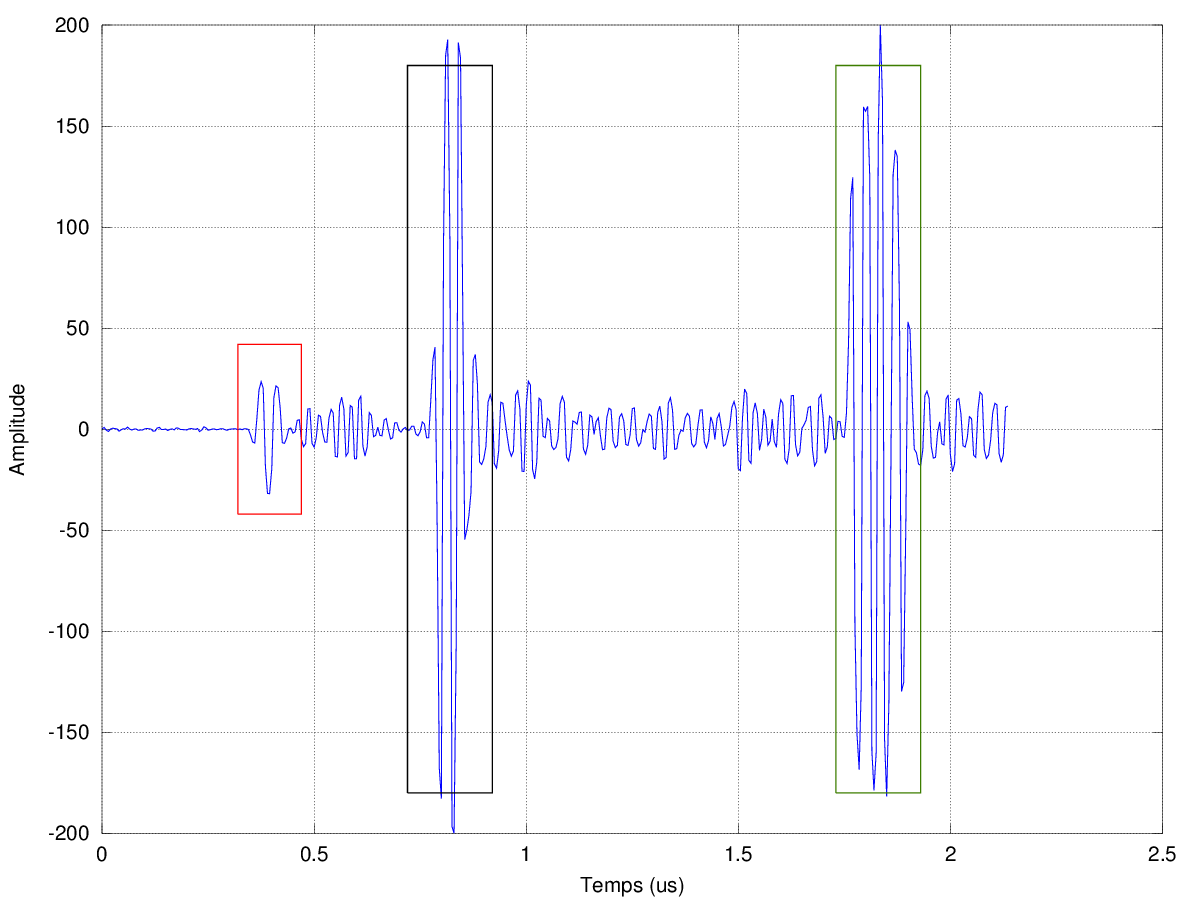
\includegraphics[width=.5\textwidth]{tofd_figs/ident_ondes.png}
    \caption{Les zones encadrées correspondent chacun à une onde différente. En rouge,
		l'onde de tête se propageant le long de l'interface a la vitesse longitudinale (à
		gauche). En noir l'onde longitudinale (à droite). En vert, l'onde transversale.}
    \label{tofd:ident_ondes}
\end{figurehere}

\subsection{Mesure en plaque saine}

Un B-Scan en plaque saine est réalisé et présenté en figure~\ref{tofd:bscan_saine}. Les temps d'arrivés pour chacune des deux ondes ne changent pas tout au long du scan : cela confirme l'hypothèse d'un pan de plaque sans défaut.

\begin{figurehere}
    \centering
    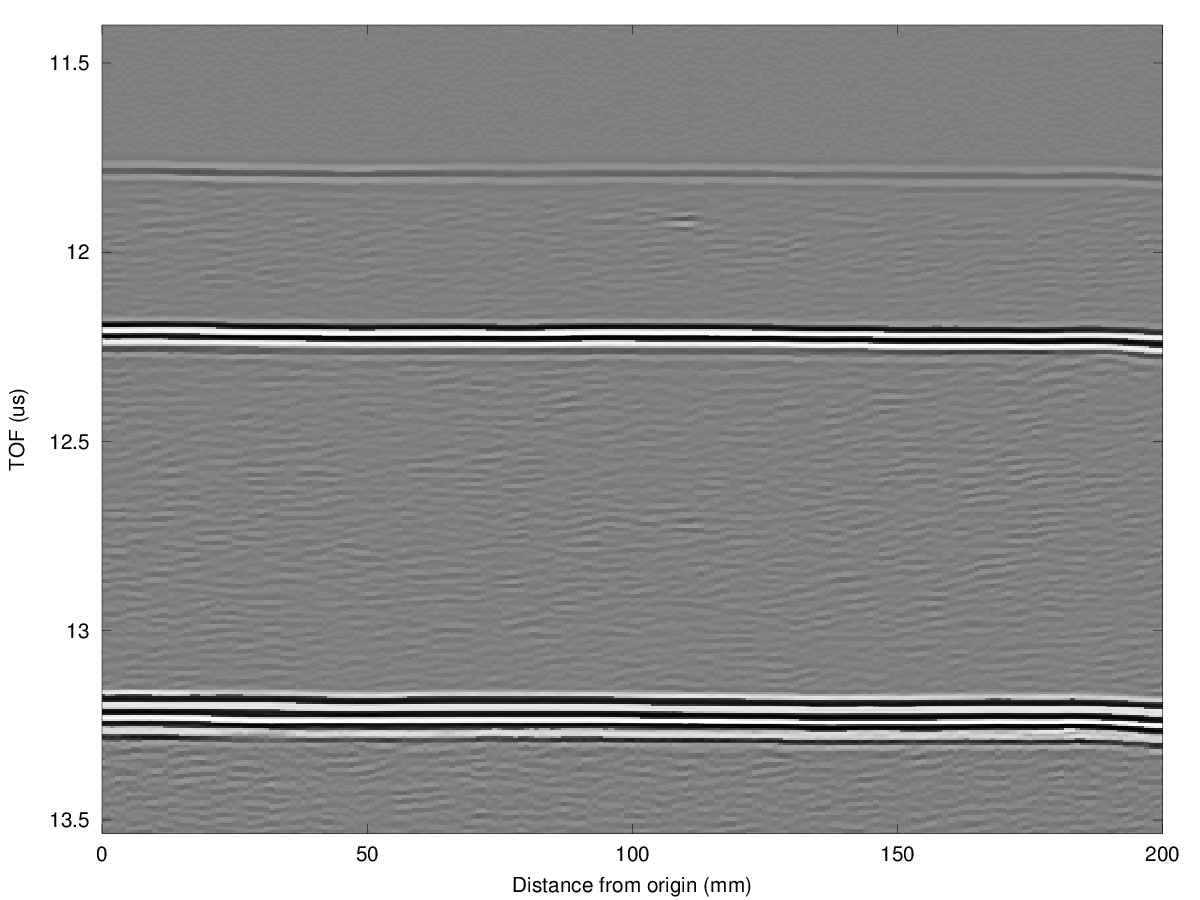
\includegraphics[width=.5\textwidth]{tofd_figs/bscan_plaque_saine.png}
    \caption{B-Scan utilisant la méthode TOFD dans une plaque saine. Tout au long du scan, les ondes longitudinales et transversales arrivent toujours aux mêmes instants : il n'y a pas de défaut ou d'élément dans l'échantillon pouvant provoquer une réflexion précoce.}
    \label{tofd:bscan_saine}
\end{figurehere}

\subsection{Mesure sur la soudure}

La méthode TOFD est utilisée pour détecter des défauts dans des plaques et des cordons de soudure.

L'objectif de cette mesure est de vérifier que TOFD permet bien la détection et le positionnement de défauts (connus ici) dans un cordon de soudure.

\subsubsection{Défauts présents}

\begin{figurehere}
    \centering
    \begin{tikzpicture}
        \draw[thick] (-3,0) -- (-0.6,0) -- ++(.5,.5) -- ++(0,.2) -- ++(-.5,.5) -- (-3,1.2);
        \begin{scope}[xscale=-1]
            \draw[thick] (-3,0) -- (-0.6,0) -- ++(.5,.5) -- ++(0,.2) -- ++(-.5,.5) -- (-3,1.2);
        \end{scope}

        % center line crack
        \draw[thick] (-.8,1.2) .. controls (-.3,1.4) and (.3,1.4) .. (.8,1.2);
        \draw[thick] (-.8,0) .. controls (-.3,-.2) and (.3,-.2) .. (.8,0);

        % root fusion
        \draw[very thick] (-.05,.6) ++(-45:.4) -- ++(-45:.3);
        \draw[very thick] (0,.8) .. controls (-.1,1) and (.1,1) .. (0,1.2);

        % porosity
        \draw (.05,.1) circle (.05);
        \draw (.07,.25) circle (.05);
        \draw (-.05,.2) circle (.05);

				\node (crack) at (.2,1.1) {1};
				\node (fusion) at (.5,.4) {2};
				\node (porosity) at (-.25,.1) {3};
		\end{tikzpicture}
    \caption{Localisation des défauts au sein du cordons, coupe transversales avec projeté (reproduction depuis la documentation).}
    \label{tofd:fig:defects}
\end{figurehere}

\begin{tablehere}
\centering
\begin{tabular}{c|c|c|c}
Numéro & Type & Taille & Position \\ \hline
1 & Fissure médiane & 21 & 46 \\
2 & Manque de fusion & 25 & 147 \\
3 & Porosité & 27 & 213
\end{tabular}
\caption{\label{tofd:tab:defects} Type, position et taille (en mm) des défauts au sein de la soudure.}
\end{tablehere}

\subsubsection{Éxpérience}

Un B-Scan est réalisé le long de la soudure afin d'essayer de positionner les défauts, le
résultat est visible en figure~\ref{tofd:fig:weld}.

\begin{figurehere}
	\centering
	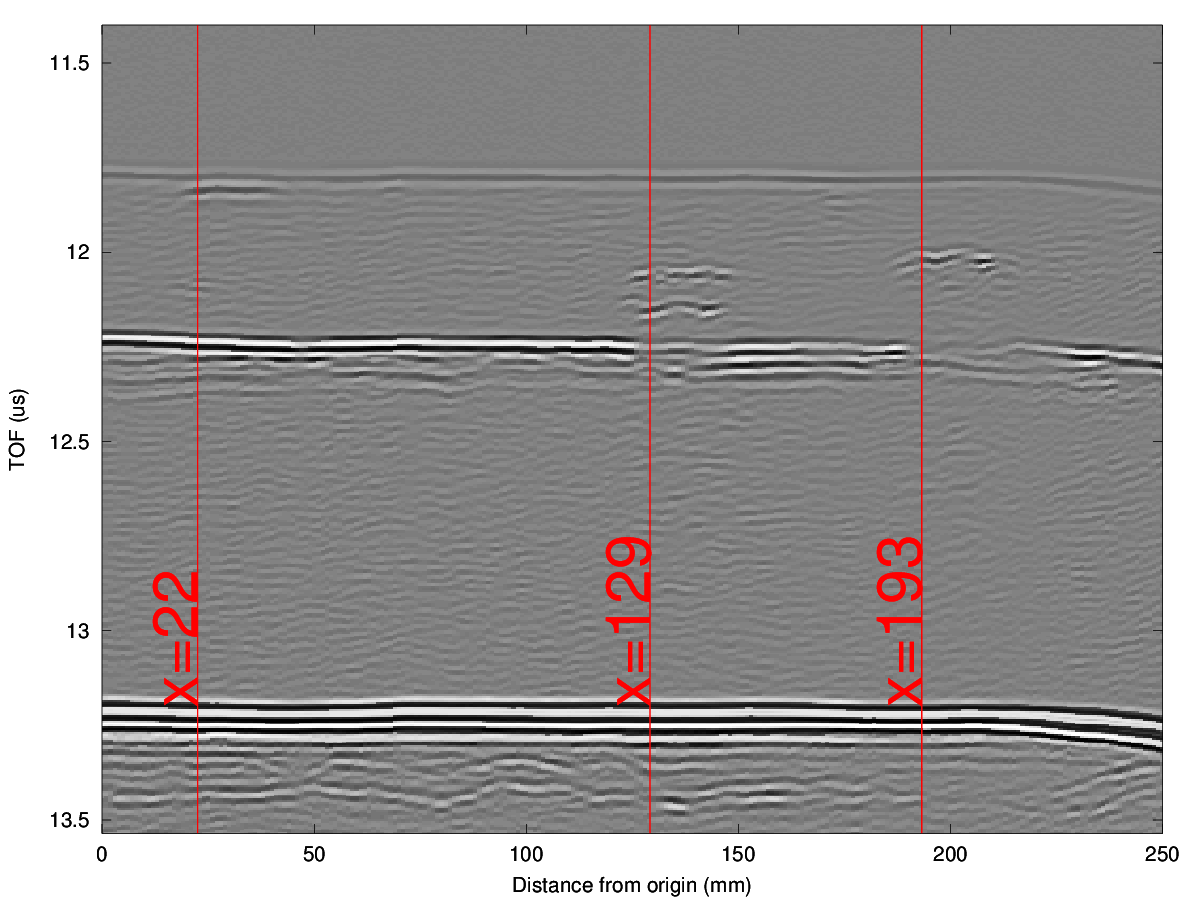
\includegraphics[width=0.8\linewidth]{tofd_figs/soudure.png}
	\caption{B-Scan le long de la soudure, les modifications de l'écho sont marquées en
	rouge. Ces modifications apparaissent pour $x=21mm$, $x=129mm$ \& $x=192mm$.}
	\label{tofd:fig:weld}
\end{figurehere}

L'écart entre les positions indiquées par la documentation liée à la plaque d'essai et
celles mesurées est assez important. Le manque d'expérience des manipulateurs est
probablement à blâmer et le mauvais calage de l'origine lors de la mesure n'améliore rien.

Des réflexions précoces sont toutefois bien visibles et il est possible en travaillant
mieux les aspects pratiques de la mesure d'obtenir un positionnement précis des défauts
dans une pièce.

\subsection{Caractérisation de la plaque par deux mesures}

La détermination de l'épaisseur de la plaque et de la vitesse de propagation au sein de
celle-ci est parfois complexe. Disposer d'une méthode permettant de déterminer rapidement
ces deux quantités est donc un avantage.

Comme suggéré par Kim \textit{et coll.}\autocite{kim_simultaneous_2003}, deux mesures à
deux distances inter-transducteurs différentes sont nécessaires pour accèder aux paramètres d'intérêt.

\begin{figurehere}
	\centering
	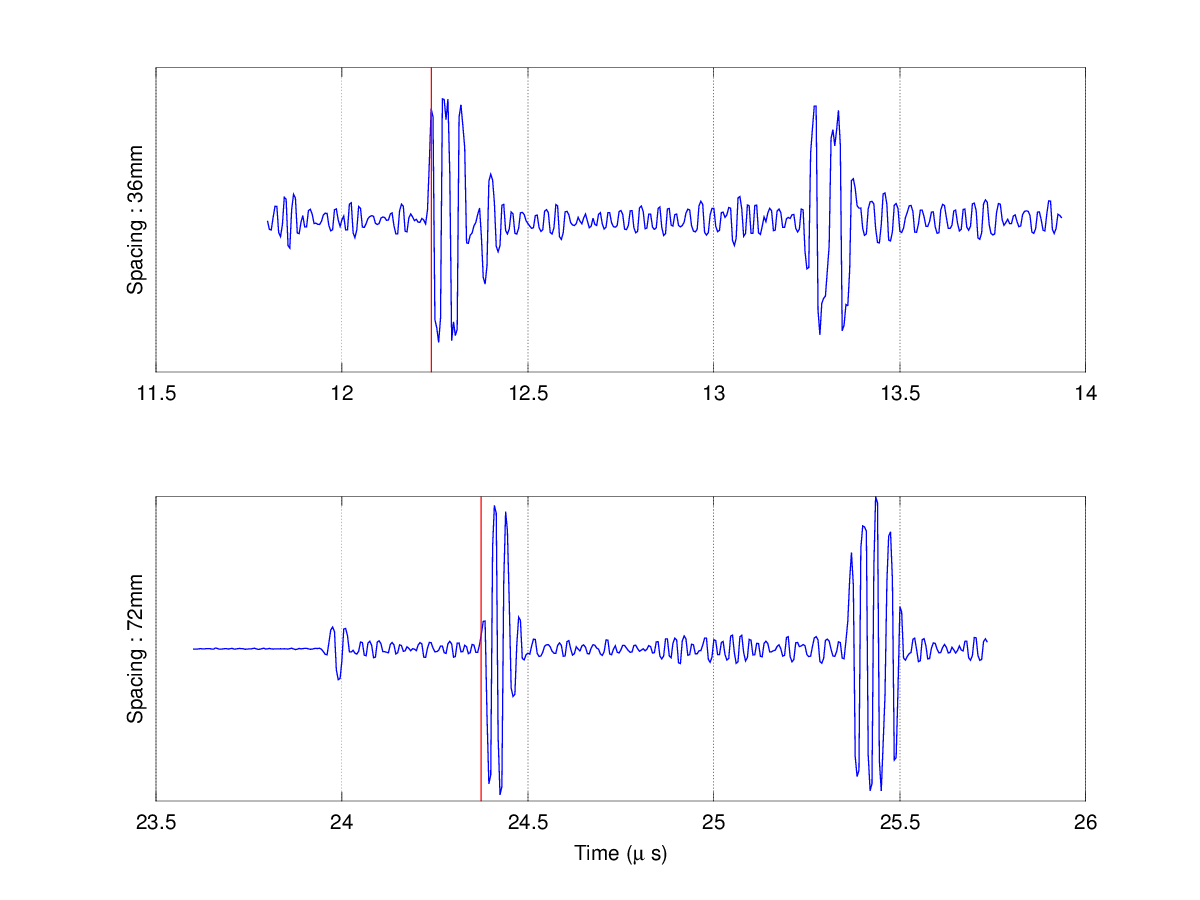
\includegraphics[width=0.8\linewidth]{tofd_figs/time_records_publi.png}
	\caption{Traces des deux signaux mesurés (attention, les abscisses ne concordent pas) pour
	la détermination simultanée de l'épaisseur et de la vitesse de propagation.}
	\label{tofd:fig:traces_publi}
\end{figurehere}

\begin{table}
	\centering
	\caption{Temps de vols et distances inter-transducteurs relevé pour la mesure
	simultannée de l'épaisseur et de la vitesse de propagation.}
	\label{tofd:tab:publi}
	\begin{tabular}{c|c}
		Distance ($mm$) & Temps de vol ($\mu s$)\\\hline
		36 & 12.25\\
		72 & 24.38\\
	\end{tabular}
\end{table}

Les signaux relevés ainsi que les temps mesurés sont présentés en
Figure~\ref{tofd:fig:traces_publi} et en Table~\ref{tofd:tab:publi}. En utilisant les
équations (3) et (4) de \cite{kim_simultaneous_2003} (reproduites en~\eqref{tofd:kim_d}
et~\eqref{tofd:kim_v}), les valeurs d'épaisseur et de vitesse de propagations sont
retrouvées (voir~\eqref{tofd:result_d} \&~\eqref{tofd:result_v}).

\begin{equation}
	d = \frac{1}{2}\sqrt{\frac{L_2^2T_1^2 - L_1^2T_2^2}{T_2^2 - T_1^2}} \label{tofd:kim_d}
\end{equation}

\begin{equation}
	v = \sqrt{\frac{L_2^2 - L_1^2}{T_2^2 - T_1^2}} \label{tofd:kim_v}
\end{equation}

\begin{equation}
	d \approx 19.4mm \label{tofd:result_d}
\end{equation}

\begin{equation}
	v \approx 2960 m\cdot s^{-1} \label{tofd:result_v}
\end{equation}

Les erreurs commises par rapport aux valeurs théoriques d'épaisseur et de vitesse sont
respectivment de 7.24\% et 7.60\%. Le fait que les deux erreurs soient si proches indique
que le facteur d'imprecision est probablement le même pour les deux. La méthode est
suffisament précise pour donner de bon résultats attendu que la mesure des temps de vol et
de la distance inter-tranducteur soit bonne.

\section*{Conclusion}

Ce TP a permis de comprendre le principe de fonctionnement de la méthode TOFD tant pour le
positionnement de défaut que pour des applications annexes de mesure d'épaisseur ou de
vitesse de propagation.

Concrètement, la force de cette méthode est sa facilité de mise en oeuvre et son faible
coût. Elle est adaptée à des applications diverses sans demander une longue formation du
manipulateur.


\part{Ondes de Lamb \& Transducteurs EMAT}
\setcounter{section}{0}
Le but de ce TP est d'étudier différentes structures au moyen d'ondes de Lamb.
L'objectif premier est de comprendre la génération des ondes de Lamb (au moyen d'un
faiseau ultrasonore d'une part et de la technologie EMAT\footnote{ElectroMagnetic Acoustic
Transducer} d'autre part), l'objectif second est de déterminer comment ces ondes peuvent être utilisées pour détecter des défauts dans des structures complexes.

Ce TP se décompose ainsi en trois parties :
\begin{enumerate}
    \item Approche théorique du phénomène
    \item Mesure des ondes de Lamb sur une plaque
    \item Positionnement de défauts sur une conduite par ondes de Lamb
\end{enumerate}

\section{Ondes de Lamb -- Élements de Théorie}

Les ondes de Lamb sont des ondes se propageant dans toute l'épaisseur d'une plaque, leurs multiples réflections sur les surfaces de la plaque en font un outil précieux pour la détection de défaut.

Ces ondes présentent deux comportements modaux distincts\footnote{Symétrique et Antisymétrique} et répondent à l'équation~\eqref{emat:eq_lamb}.
En cherchant les racines de chacun des deux termes de l'équation, il est possible d'obtenir les courbes de dispersion des différents modes et donc de savoir lesquels sont excités pour une fréquence donnée.

\begin{floatEq}
    \begin{equation}
        \begin{array}{c}
        \overbrace{
        \left[4k_x^2k_{z_L}k_{z_T}\cos\left( k_{z_L}\frac{h}{2}\right)\sin\left(k_{z_T}\frac{h}{2}\right) +\left( 2k_x^2-k_T^2\right) ^2\cos\left( k_{z_T}\frac{h}{2}\right)\sin\left( k_{z_L}\frac{h}{2}\right) \right]}^{\mathrm{modes~symétriques}}\\
        \cdot\underbrace{\left[4k_x^2k_{z_L}k_{Z_T}\cos\left( k_{z_T}\frac{h}{2}\right) \sin\left( k_{z_L}\frac{h}{2}\right) +\left( 2k_x^2-k_T^2\right) ^2\cos\left( k_{z_L}\frac{h}{2}\right) \sin\left( k_{z_T}\frac{h}{2}\right) \right]}_{\mathrm{modes~antisymétriques}}=0
        \end{array}
        \label{emat:eq_lamb}
    \end{equation}
\end{floatEq}

Les courbes de dispersion pour une plaque d'aluminium (dont les paramètres sont disponibles en table~\ref{emat:params_alu}) sont présentées dans le plan $(fh,v_\phi)$ en Figure~\ref{emat:disper_alu}.

\begin{figure}
	\centering
	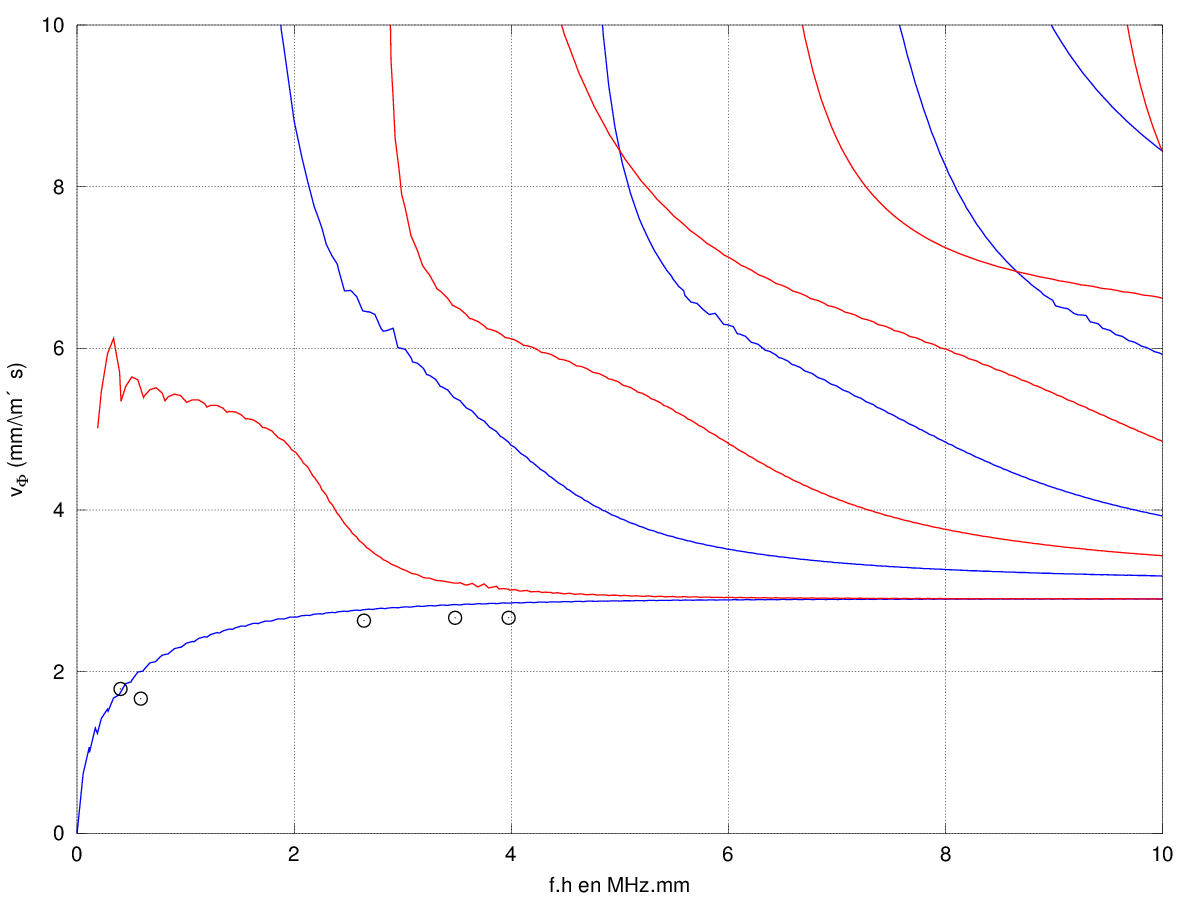
\includegraphics[width=0.8\linewidth]{me_figs/dispercurves_aluminium.png}
	\caption{Courbes de dispersion théoriques pour une plaque d'aluminium de 5.6mm
	d'épaisseur. Les modes symétriques sont en bleu, les antisymétriques en rouge. Les
	marques noires correspondent aux mesures présentées en~\ref{emat:sec:oscillo}.}
	\label{emat:disper_alu}
\end{figure}

La théorie de Lamb~\autocite{lamb_waves_1917} a été développée pour des plaques infinies
dans le plan, plongées dans le vide. La propagation d'ondes de Lamb dans une plaque finie induit des réflexions sur les bords de la plaque. Ces ondes réfléchies forment une traînée diffuse lors de la mesure. Il est par conséquent difficile (voir~\ref{emat:sec:oscillo}~) de mesurer et suivre les différentes ondes se propageant. Afin de simplifier l'étude expérimentale, seule une fenêtre assez courte est considérée pertinente (avant que les modes ne s'entre-masquent).


\begin{table*}[t]
    \centering
    \begin{tabular}{l|cc}
        Paramètre & Valeur & Unité\\\hline
        Vitesse de l'onde longitudinale dans l'acier $v_L$ & $6450$ & $m.s^{-1}$\\
        Vitesse de l'onde transversale dans l'acier $v_T$ & $3100$ & $m.s^{-1}$\\
        Épaisseur de la plaque $e$ & $5.6\cdot 10^{-3} \pm 0.1\cdot 10^{-3}$ & $m$\\
    \end{tabular}
    \caption{Paramètres de la plaque en aluminium.}
    \label{emat:params_alu}
\end{table*}

\section{Mesure des ondes de Lamb sur une plaque}
\subsection{Montage}

Les transducteurs disponibles étaient centrés à 0.5MHz et 1MHz.

Dans un premier temps, les ondes étaient générées à l'aide d'un transducteur placé au contact\footnote{Avec du couplant} de la surface, en incidence normale.
La condition de fenêtre d'analyse courte évoquée plus haut impose que la distance entre les transducteurs ne soit pas trop grande.

\begin{figurehere}
\begin{tikzpicture}[>=stealth]
    \def\platehalfwidth{3}
    \newcommand\transducer[2]{
        \draw[thick] (#1+0,0) rectangle ++(.3,.4);
        \draw[thick] (#1+.15,.4) .. controls (#1+.2,.7) and (#1+.3,.7) .. (#1+.3,1);
        \draw (#1+.15,0) node[below] {#2};
    }
    \newcommand\inp[3]{
        \draw (0+#1,0+#2) -- ++(.2,0) -- ++(-.1,.2) -- cycle;
        \draw (.3+#1,.6+#2) node[rotate=90, above] {#3};
    }

    % part
    \draw[very thick] (-\platehalfwidth,0) -- (\platehalfwidth,0);
    \draw[very thick] (-\platehalfwidth,-1) -- (\platehalfwidth,-1);
    \draw[very thick] (-\platehalfwidth,0) .. controls (-\platehalfwidth-.5,-.5) and (-\platehalfwidth+.5,-.5) .. (-\platehalfwidth,-1);
    \begin{scope}[shift={(2*\platehalfwidth,0)}]
        \draw[very thick] (-\platehalfwidth,0) .. controls (-\platehalfwidth-.5,-.5) and (-\platehalfwidth+.5,-.5) .. (-\platehalfwidth,-1);
    \end{scope}

    % transducers
    \transducer{\platehalfwidth{}-1.5}{$TX$}
    \transducer{\platehalfwidth{}-4}{$RX_1$}
    \transducer{\platehalfwidth{}-5.5}{$RX_2$}

    % distances
    \draw[<->] (\platehalfwidth-4,.2) -- ++(-1.2,0)  node[midway, above] {$25mm$};
    \draw[<->] (\platehalfwidth-1.5,.2) -- ++(-2.2,0)  node[midway, above] {$50mm$};

    % GBF
    \draw[very thick] (.5,2.5) -- ++ (0,-.5) -- ++(2,0) -- ++(0,.5) node[midway, right] {GBF};
    \inp{1}{2}{SYNC}
    \inp{1.7}{2}{OUT}

    % Oscillo
    \draw[very thick] (-1.8,2.5) -- ++ (0,-.5) node[midway, left] {Oscilloscope} -- ++(2,0) -- ++(0,.5);
    \inp{-.3}{2}{TRIG}
    \inp{-0.8}{2}{CH1}
    \inp{-1.3}{2}{CH2}

    % cables
    \draw[thick] (1.1,2) -- ++(0,-.3) -- (-.2,1.7) -- ++(0,.3);
    \draw[thick] (1.8,2) -- (1.8,1);
    \draw[thick] (-.7,1) -- (-.7,2);
    \draw[thick] (-2.2,1) -- ++(0,.5) -- (-1.2,1.5) -- ++(0,.5);

    % dimensions
    \draw[<->] (2.5,0) -- ++(0,-1) node[midway, right] {$e$};
\end{tikzpicture}
\caption{\label{emat:dispositif_plaque}Dispositif de mesure de la vitesse de propagation des différents modes de Lamb dans une plaque avec un oscilloscope et un générateur de signaux.}
\end{figurehere}

\subsection{Mesures à l'oscilloscope}\label{emat:sec:oscillo}

Le signal d'excitation utilisé est un \textit{burst}, de 3 cycles de sinusoïde sur une fenêtre de 10ms.

L'utilisation d'une période de répétition du \textit{burst} assez grande permet de
s'affranchir des problèmes liés à la superposition de signaux d'excitation. Dans toutes
les mesures, l'ensemble du train d'ondes ne couvrait pas plus de 5 à 10\% de la période de
répétition totale.

En superposant les signaux venant de $RX_1$ et $RX_2$ sur l'oscilloscope il est alors
possible de mesurer le temps de parcours du signal entre les deux récepteurs et de
remonter alors à la vitesse de propagation (vitesse de phase) pour chacun des mode
distingables.

Le système expérimental en place, différentes mesures de temps de vol entre $RX_1$ et
$RX_2$ à différentes fréquences sont réalisées.


La vitesse de chacun des modes de Lamb dépend grandement de la fréquence. De même, dans
l'espace $(fh,v_\phi)$, les courbes de dispersion s'entre-croisent : sans
connaissance \textit{a priori} de ces courbes, il n'est pas possible d'identifier un mode
particulier (l'orde d'arrivée change).

De plus, avec l'augmentation de la fréquence, les vitesses des différents modes convergent vers la même asymptote. Si au début de l'analyse il est possible d'observer des ondes bien séparées, cela devient vite impossible et un seul paquet est observable sans que des modes particuliers soient vraiment distingables.

Les résultats les plus probants des mesures réalisées sont présentés sous forme de cercles
noirs sur la figure~\ref{emat:disper_alu}.

L'adéquation entre la courbe de dispersion et le mode S0 est plutôt bonne mais les autres
mesures étaient toutes largement en dessous de l'asymptote commune.

La mesure précise d'ondes de Lamb avec un oscilloscope est un exercice complexe notamment
à cause des variations importantes de vitesse en fonction de la fréquence et de
l'épaisseur.

Dans la suite un système EMAT sera utilisé. Ces éléments ont notamment l'énorme avantage
de pouvoir générer un mode de Lamb particulier plutôt que tous les modes en même temps
(comme c'était le cas précédement).

\section{Mesures EMAT}

La méthode de mesure utilisée dans la suite est basée sur le système EMAT\footnote{\textit{Electromagnetic Acoustic Transducer}}. Le principe est de générer des ondes acoustiques dans un matériau ferro-magnétique au moyen d'un champ electromagnétique.

Le système EMAT se compose donc d'un chariot porteur d'une bobine au pas calibré pour exciter certains modes de la pièce et d'un odomètre. Le tout est relié a un boîtier de contrôle et, éventuellement à un ordinateur pour automatiser les acquisitions et faciliter le traitement.

Dans le cas présent, le logiciel de contrôle (et d'export) normalement disponible sur l'ordinateur associé n'était pas fonctionnel. Le système chariot/boîtier a pour seul format de sortie des fichiers .dat qui s'avèrent être des binaires non documentés.

Malgré beaucoup de bonne volonté, tous les efforts pour accèder aux données présentes dans le binaire se sont montrés quasi-infructueux. Au mieux, il a été possible de récupérer des méta-données sur l'acquisition et une forme de signal temporel sans indice d'échelle temporelle ou en amplitude.

Sans pouvoir faire mieux dans le temps imparti, l'option choisie est de ne pas considérer les mesures réalisées et de proposer simplement un protocole possible pour détecter et positionner des défauts au moyen d'un système EMAT dans une pièce cylindrique.

\subsection{Interaction entre défauts et ondes}

Les ondes de Lamb se propagent dans toute l'épaisseur du matériau et leur vitesse de phase dépend de cette épaisseur (voir équation~\eqref{emat:eq_lamb} et noter la dépendance en $h$). La présence d'un défaut modifie l'épaisseur (corrosion, fissure débouchante) ou induit une discontinuité dans l'espace de propagation (fissure non-débouchante).

Dans le second cas, la discontinuité provoque une réflexion de l'onde visible sur la trace
temporelle (voir figure~\ref{emat:ondes_conduite}). Dans le premier cas, la modification de l'épaisseur change la constante de propagation (liée à la vitesse) et par conséquent provoque un changement d'impédance plus ou moins brusque et donc une réflexion plus ou moins marquée.

Dans ces deux cas, la conclusion est qu'une réflexion dans la trace est liée à un défaut. Exception doit être faite toutefois des discontinuités liées à des composantes géométriques particulière (épaulements, perçages, etc...) que l'opérateur consciencieux prendra bien évidemment en considération dans son analyse.

\begin{figure}
	\centering
	\begin{tikzpicture}
		% tube
		\draw[very thick] (0,0) circle (1.5);
		\draw[very thick] (0,0) circle (1.7);

		% EMAT
		\draw[thick] (105:1.75) arc (105:75:1.75) -- ++(0,.7) -- ++(-.9,0) node[midway, above] {EMAT} -- ++(0,-.7);

		% crack
		\draw[very thick] (-45:1.5) -- (-47:1.7);
		\draw[thin] (-46:1) -- (-46:2.5) node[right] {Défaut};

		% ondes horaires
		\draw[dashed, blue,->] (73:1.85) arc (73:-45:1.85);
		\draw[dashed, blue,<-] (73:2) arc (73:-45:2);

		% onde anti-horaires
		\draw[dashed, red,->] (107:1.85) arc (107:313:1.85);
		\draw[dashed, red,<-] (107:2) arc (107:313:2);

	\end{tikzpicture}
	\caption{Des ondes de Lamb se propagent au sein de la conduite de par et d'autre de
	l'EMAT. Le défaut produit une réflexion précoce et sur la base des temps de vol
	aller-retour il peut être positionné.}
	\label{emat:ondes_conduite}
\end{figure}

\paragraph{Position relative chariot/défaut}
Le temps de vol de l'onde réfléchie renseignant sur la distance entre le chariot de mesure et le défaut, il est alors logique que deux mesures (loin des défauts) suffisent à détecter et positionner un défaut.

Cette clause portant sur le fait que le chariot ne soit pas positionné sur ou trop proche d'un défaut est liée à l'existence de zones mortes (comme pour la méthode TOFD\footnote{\textit{Time Of Flight Difraction}}).
Contrairement au cas le plus idéal, l'émission du signal d'excitation n'est pas un évènement infiniment court et l'émission masque, pendant un temps significatif, toute réflexion précoce.

Afin de s'affranchir de ce problème, il est envisageable de réaliser trois et non deux mesures sur la pièce à des angles différents et d'opérer un recoupement des données ensuite. Le choix des angles doit se faire en considérant la géométrie de la pièce, ses défauts éventuellement visibles, etc. Il sera peut être également nécessaire d'envisager des angles réparti inégalement ou même de refaire des mesures plus précise autour de défauts détectés pour affiner l'analyse.

\paragraph{Différents Modes}
Différents modes de Lamb se propagent \textit{a priori} à différentes vitesses (jusqu'à une certaine fréquence)  et n'induisent pas les mêmes contraintes internes. Par conséquent, différents modes ne réagiront \textit{a priori} pas de la même manière avec différents défauts. Il est alors judicieux de réaliser des mesures en excitant différents modes.

\subsection{Mode Opératoire}

Considérant les différents points évoqués au paragraphe précédent le mode opératoire pour un contrôle de conduite par EMAT pourrait être :

\begin{enumerate}
    \item Analyser la géométrie de la pièce et déterminer 3 axes possibles pour l'avance du chariot sur toute la longueur de la section à contrôler.
    \item Opérer une mesure blanche pour contrôler le bon fonctionnement du système sur une pièce (ou une section) considérée saine.
    \item Réaliser une mesure sur chacun des axes d'avance prévus, noter les angles relatifs entre les passes.
    \item Refaire une mesure par axe pour au moins deux autres modes de Lamb.
    \item Afficher des images d'ensemble pour chaque mode de Lamb excité et constater la position des défauts.
    \item Refaire des mesures autour des défauts avec différents modes de Lamb pour améliorer la caractérisation du défaut.
\end{enumerate}

\newpage

\section*{Conclusion}

Les ondes de Lamb présentent un grand nombre d'intérêts ; en effet leur sensibilité aux changements d'épaisseur du milieu de propagation est un avantage considérable pour le CND appliqué à des conduites.

L'utilisation de systèmes EMAT permet d'exciter un mode particulier du système sans action mécanique sur la pièce. Ce point est particulièrement avantageux dans le cas de systèmes critiques où un dommage minime peut avoir des conséquences dramatiques (\textit{pipelines}, conduites chimiques etc.).

La précision que démontrent les EMAT dans la génération de modes particuliers du système pourrait être couplée à des techniques de traitement de signal avancé pour la détection de forme. En ajoutant à l'équation un système expert avec apprentissage supervisé, il serait peut être possible d'aboutir à un outil capable de mesurer et caractériser automatiquement des défauts qui ne demanderait qu'un minimum d'action humaine.
Cette optique prend tout son sens dans le cas de système de SHM\footnote{Structure Health Monitoring}.


\part{Ondes de Volumes/Ondes de Surface}
\setcounter{section}{0}
L'objectif de cette section est de comprendre et expérimenter la génération de différents types d'ondes dans un solide isotrope.

Dans la suite plusieurs manipulations sont réalisées :

\begin{itemize}
    \item mesures en mode écho \& mesure de la vitesse des ondes longitudinales (A-Scan)
    \item mesures en transmission \& évaluation de l'influence de l'angle d'incidence
    \item mesures de la vitesse d'ondes de surface en mode écho et transmission latérale
    \item mesures du re-rayonnement associé à la propagation d'une onde de Rayleigh généralisée\footnote{\textit{Leaky Rayleigh Wave}}
\end{itemize}

\section{Analyse théorique}

\label{volsurf:theo}

En premier lieu, il convient d'examiner les différents angles critiques à l'interface plexiglas/aluminium. Les paramètres des deux matériaux sont regroupés en table~\ref{volsurf:params}.

\begin{table*}[h]
    \centering
    \begin{tabular}{l|cc}
        Paramètre & Valeur & Unité\\\hline
        Vitesse de l'onde longitudinale dans l'aluminium $v_L$ & $6450$ & $m.s^{-1}$\\
        Vitesse de l'onde transversale dans l'aluminium $v_T$ & $3100$ & $m.s^{-1}$\\
        Vitesse de l'onde longitudinale dans le plexiglas $\tilde{v_L}$ & $2700$ & $m.s^{-1}$\\
        Vitesse de l'onde transversale dans le plexiglas $\tilde{v_T}$ & $1100$ & $m.s^{-1}$\\
        Épaisseur de la plaque $e$ & $20\cdot 10^{-3} \pm 0.1\cdot 10^{-3}$ & $m$\\
    \end{tabular}
    \caption{Paramètres remarquables de la manipulation.}
    \label{volsurf:params}
\end{table*}

\subsection{Angles Critiques}

D'après la loi de Snell-Descartes~\eqref{volsurf:snell}, viennent les calculs des angles incidents critiques (pour lesquels l'angle réfracté vaut 90\degre) en équations~\eqref{volsurf:Lcrit} &~\eqref{volsurf:Tcrit}.

\begin{equation}
    \frac{\sin \theta_1}{v_1} = \frac{\sin\theta_2}{v_2} \label{volsurf:snell}
\end{equation}

\begin{equation}
    \theta_{L_crit} = \arcsin\frac{\tilde{v_L}}{v_L} \overset{AN}{\approx} 24.7\deg \label{volsurf:Lcrit}
\end{equation}

\begin{equation}
    \theta_{T_crit} = \arcsin\frac{\tilde{v_L}}{v_T} \overset{AN}{\approx} 60.6\deg \label{volsurf:Tcrit}
\end{equation}

Les ondes se propageant dans une couche solide (aluminium) entre deux milieux solides de même nature (sabot en plexiglas), les calculs montrent que l'angle de sortie sera le même que l'angle d'entrée.

Pour optimiser la réception, il est judicieux d'orienter le transducteur de réception de manière analogue à celui d'émission. Il pourra également être nécessaire de décaler légèrement les transducteurs l'un par rapport à l'autre afin de bien centrer la réception sur le point d'émergence du faisceau en sortie de la couche métallique.

\subsection{Angle de Rayleigh}
\label{volsurf:theo:rayleigh_angle}

Les ondes de Rayleigh sont des ondes de surface se propageant à une vitesse inférieure à celle de l'onde transversale. 

Leur intérêt principal dans le cas du CND est la détection de défauts subsurfaciques où elles excellent à contrôler une zone souvent masquée dans le cadre d'autres méthodes (zone morte).

\paragraph{Équation de Rayleigh} En introduisant les nombres adimensionnels $\xi = \nicefrac{v_T}{v_L}$ et $\eta = \frac{v_R}{v_T}$ (où $v_R$ est la vitesse de propagation des ondes de Rayleigh), l'équation de Rayleigh s'exprime telle qu'en ~\eqref{volsurf:rayleigh_eq}.

\begin{equation}
    \eta^6 - 8\eta^4 + 8\eta^2(3-2\xi)^2 + 16(\xi^2-1) = 0 \label{volsurf:rayleigh_eq}.
\end{equation}

La solution approchée la plus utilisée pour déterminer la vitesse de propagation des ondes
de Rayleigh, dénommée solution de Viktorov~\autocite{viktorov_rayleigh_1970}), est proposée en~\eqref{volsurf:viktorov}.

\begin{equation}
    \eta = \frac{0.718 - \xi^2}{0.75 - \xi^2} \label{volsurf:viktorov}
\end{equation}

Il vient alors, compte-tenu des paramètres du problème présenté en table~\ref{volsurf:params} :

\begin{equation}
    v_R = v_T\frac{0.718-\xi^2}{0.75-\xi^2} \overset{AN}{\approx} = 2908 m\cdot s^{-1} \label{volsurf:an_viktorov}
\end{equation}

\paragraph{Angle de Rayleigh} Connaissant la vitesse de propagation des ondes de Rayleigh et sachant qu'il s'agit d'ondes de surface (angle réfracté valant 90\degres), il est possible de calculer l'angle d'incident optimal pour générer des ondes de Rayleigh. Toujours en utilisant la relation~\eqref{volsurf:snell} il vient :

\begin{equation}
    \theta_{R} = \arcsin\frac{\tilde{v_L}}{v_R} \overset{AN}{\approx} 68.2\deg \label{volsurf:thetaR}
\end{equation}

Comme dans une vaste majorité des cas, l'angle de Rayleigh $\theta_R$ est légèrement supérieur au deuxième angle critique.

\section{Onde de volume}

\label{volsurf:vol}

L'objet de l'étude expérimentale est ici la vérification des assertions suivantes :

\begin{enumerate}
    \item il n'y a plus d'onde longitudinale transmise après le premier angle critique ;
    \item il n'y a plus d'onde transversale transmise après le second angle critique ;
    \item le matériau est isotrope, la vitesse de propagation ne dépend pas de l'angle de propagation.
\end{enumerate}

\begin{figure*}
    \centering
    \begin{tikzpicture}
    \newcommand\transwedge[1]{
        \draw[thick, fill=white] (0,0) -- ++(4,0) -- (0,4) --cycle;
        \begin{scope}[shift={(0,-.3)}, rotate around={-#1:(3.4,0)}]
            \draw[thick] (2.5,3.6) -- ++(1.8,0) -- ++(0,-1) -- ++(-1.8,0) --cycle; % moving part
            \draw[thick] (2.5,3.6) rectangle ++(1.8,1.4); % tranducer
            \draw[thick] (3.4,5) .. controls (3.2,5.5) and (3.6,5.5) .. (3.4,6); % cable
        \end{scope}
        \draw[thick, fill=white] (.4,0) -- (6.4,0) arc (0:180:3); % half circle
        \foreach \i in {0,45,60,70}{
            \begin{scope}[rotate around={-\i:(3.6,.7)}]
                \draw (3.4,.3) -- ++(0,2);
            \end{scope}
        }
    }
    
    % part
    \draw[very thick] (-7,0) -- (7,0);
    \draw[very thick] (-7,-2) -- (7,-2);
    \draw[very thick] (-7,0) .. controls (-8,-1) and (-6,-1) .. (-7,-2);
    \draw[very thick] (7,0) -- ++(0,-2);
    %\begin{scope}[shift={(14,0)}]
    %    \draw[very thick] (-7,0) .. controls (-8,-1) and (-6,-1) .. (-7,-2);
    %\end{scope}
    
    \draw[<->, >=stealth] (7.3,0) -- ++(0,-2) node[midway, right, shift={(.3,1)}, rotate=-90] {$h=20mm$};
    
    % tranducers
    \begin{scope}[shift={(-6,0)}, scale=.3, transform shape]
        \transwedge{0}
    \end{scope}
    \draw (-5,2) node[above] {a) Mode écho};
    
    
    \begin{scope}[shift={(-1,0)}, scale=.3, transform shape]
        \transwedge{30}
    \end{scope}
    \begin{scope}[shift={(-1,0)}, yscale=-1, xscale=-1, shift={(-1,2)}, scale=.3, transform shape]
        \transwedge{30}
    \end{scope}
    \draw (0,2) node[above] {b) Mode transmission};
    
    
    \begin{scope}[shift={(6,0)}, xscale=-1, scale=.3, transform shape]
        \transwedge{60}
    \end{scope}
    \draw (5,2) node[above] {c) Ondes de Rayleigh};
    
    \end{tikzpicture}
    \caption{Différents montages expérimentaux utilisés. A gauche, en mode écho, l'onde est transmise en incidence normale et renvoyée par le fond de plaque. Au centre, en mode transmission, l'onde est transmise avec une incidence $\theta_I$ et est transmise avec le même angle en sortie de plaque. À droite, le mode écho est utilisée pour la détection d'onde de Rayleigh après leur réflexion en bord de plaque.}
    \label{volsurf:montages}
\end{figure*}

\subsection{Mode écho}
\label{volsurf:vol_echo}

L'objectif ici est de comparer la vitesse théorique de l'onde de compression avec sa vitesse effective.
Le montage expérimental utilisé est la configuration a) de la figure~\ref{volsurf:montages}.
Le transducteur émet une onde longitudinale se propageant dans le plexiglas puis arrivant avec une indidence normale sur l'interface plexiglas/aluminium.
Une onde longitudinale est alors générée dans l'aluminium et réfléchie sur le fond de plaque avant de revenir au transducteur.

A l'oscillocope, les temps de vol mesurées comprendrons donc deux fois le temps de vol dans les $h_w = 3.5cm$ de plexiglas qui séparent le transducteur de la plaque ainsi que 2 fois le temps de parcours de la plaque (aller-retour).

\begin{figurehere}
    \centering
    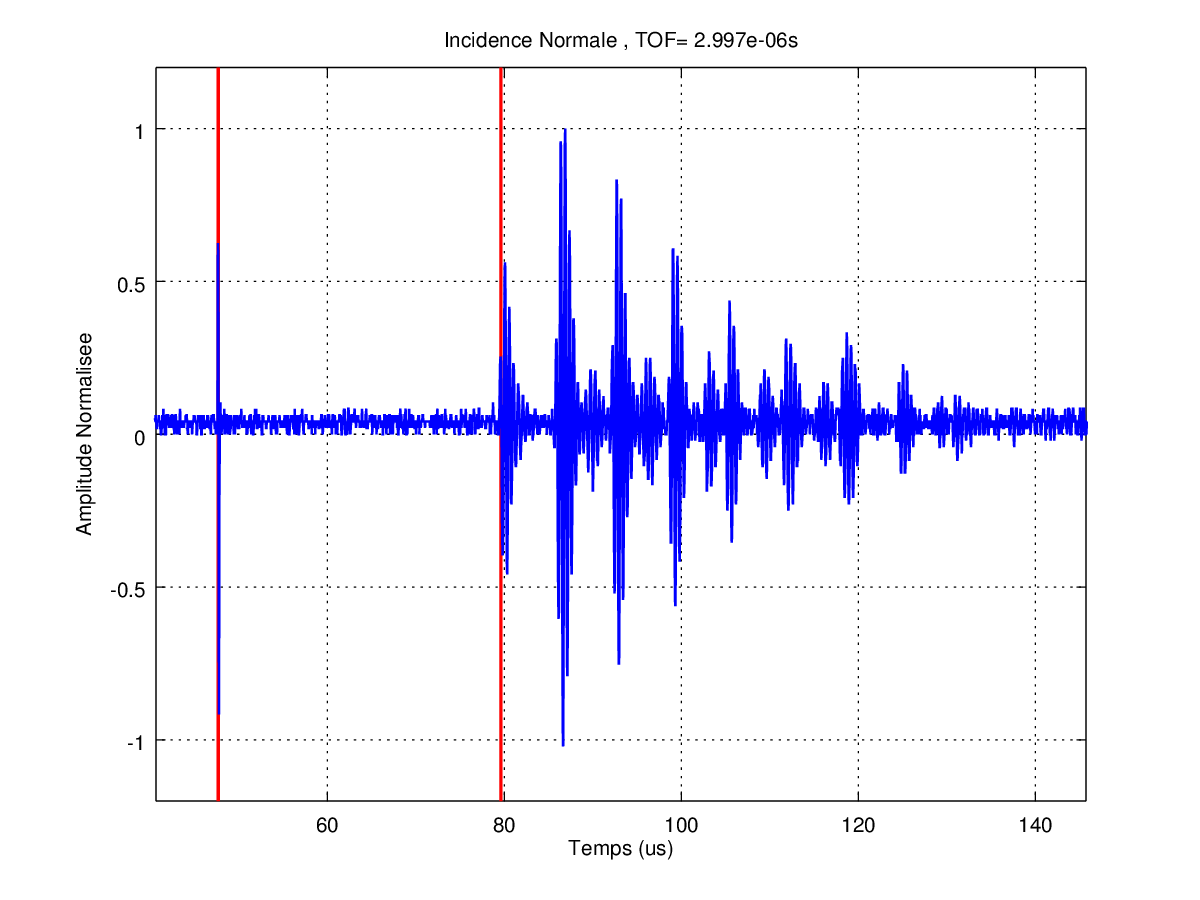
\includegraphics[width=.5\textwidth]{volsurf_figs/DS0000_incnorm.png}
    \caption{Mesure ultrasonore en mode écho. Connaissant l'écart temporel entre le signal de synchronisation (à environ $20\mu s$) et le début du premier écho (à environ $80\mu s$) il est possible de remonter à l'épaisseur de plaque (connaissant la vitesse ou \textit{vice versa}). Les calculs sont donnés au paragraphe~\ref{volsurf:vol_echo}.}
    \label{volsurf:echo_norm}
\end{figurehere}

La formule pour remonter à une estimation $\hat{v}_L$ de la vitesse des ondes longitudinales (seules excitées en incidence normale) est donnée en~\eqref{volsurf:back_to_longi} (où $\tau$ est le temps de vol relevé et $h$ l'épaisseur de la plaque). 

\begin{equation}
    \hat{v}_L = \frac{h}{\tau}
    \label{volsurf:back_to_longi}
\end{equation}

Dans le cas des paramètres utilisés et des mesures effectuées au cours de la manipulation présentée ici, la vitesse était estimée telle que : $\hat{v}_L = \approx 6673 m\cdot s^{-1}$ soit une erreur relative d'environ 3.5\%.

\subsection{Mode transmission}

Dans un second temps, le montage b) de la figure~\ref{volsurf:montages} est utilisé pour exciter à la fois des ondes longitudinales et transversales dans le volume.

Les résultats de ces mesures sont consignés en table~\ref{volsurf:speed_angles} et sont à comparer avec les valeurs théoriques de vitesses indiquées en table~\ref{volsurf:params}.  

\begin{tablehere}
    \centering
    \begin{tabular}{c|cc|cc}
         Angle & $\tau_L$ & $\hat{v}_L$ & $\tau_T$ & $\hat{v}_T$\\\hline
         0 & 6 & 3293 & & \\
         10 & 5 & 3941 & 8.6 & 2333\\
         20 & 4 & 4909 & 7.7 & 2606\\
         30 & & & 7.7 & 2606\\
         40 & & & 7.1 & 2827\\
         50 & & & 7.1 & 2827\\
    \end{tabular}
    \caption{Temps de vols et vitesses mesurés pour différents angles d'incidence sans appliquer de correction de longueur pour modéliser la réfraction du faisceau (changement de distance faibles). Les temps sont donnés en $\mu s$ et les vitesses en $m\cdot s^{-1}$, l'adéquation avec les valeurs théoriques fournies en table~\ref{volsurf:params} est plutôt mauvaise.}
    \label{volsurf:speed_angles}
\end{tablehere}

Les écarts constatables en théorie et expérience peuvent être liés à plusieurs facteurs.
Le premier est une erreur sur la mesure elle même : un mauvais couplage entre les transducteurs et la plaque, un mauvais réglage des outils de mesure, etc... autant de causes pouvant expliquer les erreurs constatées.

Un autre souci pourrait être que la plaque est véritablement anisotrope et/ou n'est pas un simple aluminium. De ce côté, plusieurs pistes sont à explorer : d'autres mesures de vitesses et de constantes mécaniques, un calcul de masse volumique, etc... pour connaître les paramètres réels de la plaque.

Ces essais ne sont pas traités ici.

\section{Onde de surface}

Cette section présente une technique de génération d'onde de surface\footnote{ici ondes de Rayleigh} dans une plaque de métal.

L'analyse cherche à vérifier les assertions :
\begin{itemize}
    \item la vitesse effective des ondes de Rayleigh est proche de celle indiquée par la solution approchée de Viktorov~\eqref{volsurf:an_viktorov} ;
    \item dans le cas de la génération d'onde de Rayleigh, il n'y a pas d'onde transmise.
\end{itemize}

L'analyse préliminaire indique (section~\ref{volsurf:theo}\ref{volsurf:theo:rayleigh_angle}) que l'angle de génération des ondes de Rayleigh est $\theta_R = 68.2\deg$.

Deux montages sont possibles :
\begin{enumerate}
    \item un unique transducteur en mode écho faisant face au bord de la plaque. L'onde est générée au niveau du transducteur, se propage le long de la surface jusqu'au borde de plaque où elle est réfléchie puis détectée (voir figure~\ref{volsurf:montages} c)~) ;
    \item deux transducteurs se faisant face sur le même côté de la plaque, réglés avec le même angle (transmission latérale).
\end{enumerate}

Seul le premier de ces deux montages est mis en œuvre ci-après pour la mesure de la vitesse de l'onde de Rayleigh (l'air baignant la plaque est assimilé a du vide et le re-rayonnement n'est pas considéré).

La section suivante s'intéressera à la génération et à la détection d'ondes de Rayleigh généralisées.

\subsection{Mode écho}

En mode écho, un unique transducteur fait face au bord de plaque séparée de celui-ci par une distance $d = 5.7cm$.

La mesure se fait de manière analogue à ce qui a été présenté en section~\ref{volsurf:vol}\ref{volsurf:vol_echo}. La trace temporelle est disponible en figure~\ref{volsurf:echo_norm}) et le calcul de vitesse donne :

\begin{equation}
    \hat{v}_R  = \frac{d}{\tau_R} = \overset{AN}{=} \frac{5.7\cdot10^{-2}}{19.2\cdot10^{-6}} \approx 2967m\cdot s^{-1}
\end{equation}

\begin{figurehere}
    \centering
    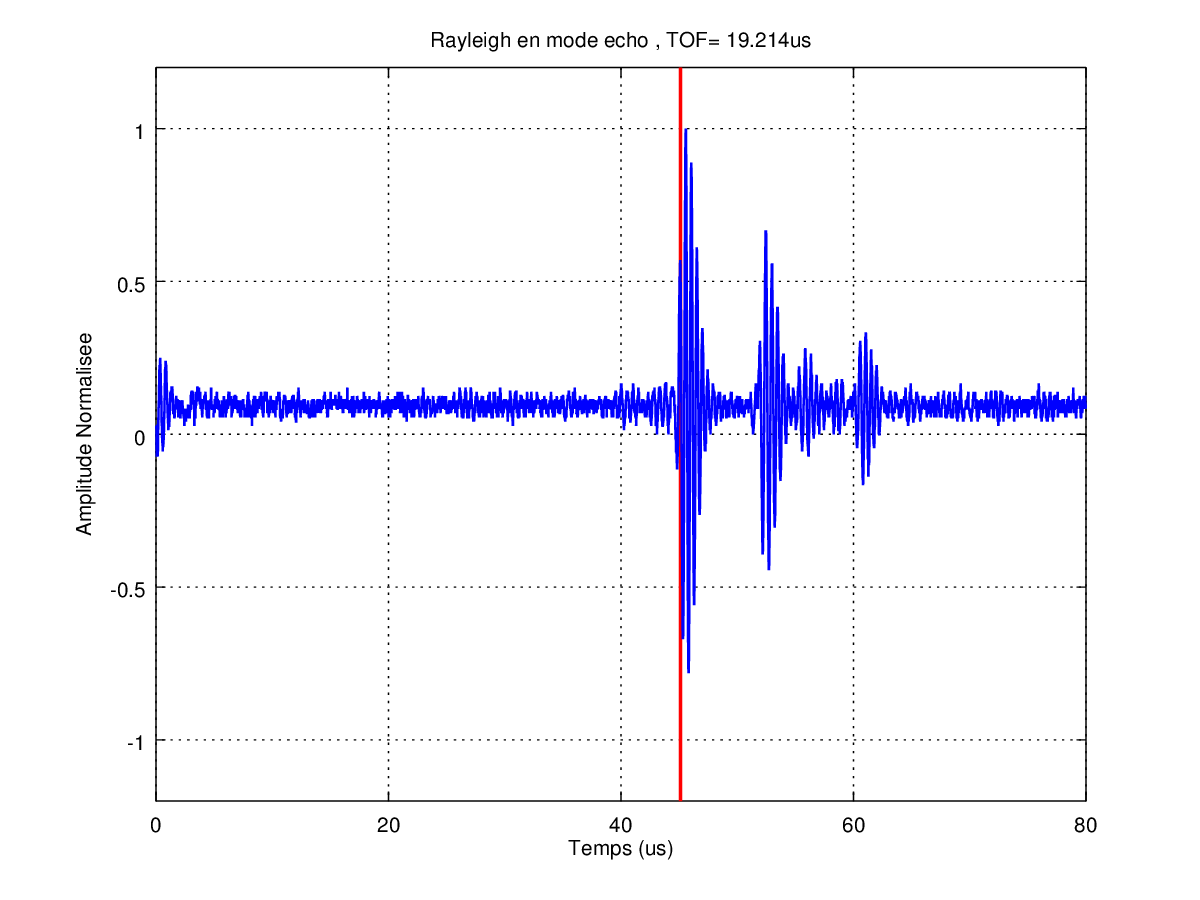
\includegraphics[width=.5\textwidth]{volsurf_figs/DS0008_rayleigh_echo.png}
    \caption{Mesure en mode écho de la vitesse des ondes de Rayleigh. la chaîne d'acquisition est paramétrée de sorte que le signal de synchronisation soit en $t=0$. Le front d'onde utilisé pour la mesure de vitesse est noté en rouge.}
    \label{volsurf:echo_norm}
\end{figurehere}

La valeur de vitesse précédente présente un écart relatif d'environ 2\% avec la valeur proposée par la solution de Viktorov (équation~\eqref{volsurf:an_viktorov}).

\subsection{Onde de surface et charge}

Les ondes de surface se propagent, comme leur nom l'indique, le long de l'interface et sont donc très sensibles à un changement de conditions limites.

Un cas bien connu est la génération d'ondes de Rayleigh généralisées mais un cas beaucoup plus simple consiste à venir poser une masse sur le trajet des ondes. Dès lors que la surface n'est plus libre, l'amplitude des ondes de Rayleigh est très fortement diminuée.

\section{Onde de Rayleigh généralisée}

Lorsque le fluide est visqueux ou simplement lorsque le couplage fluide-structure ne peut plus être négligé, il est coutume de parler d'onde de Rayleigh généralisée ou d'onde de Rayleigh de fuite\footnote{\textit{Leaky Rayleigh Wave} en anglais}. Ce nom vient du re-rayonnement d'énergie observable dans le fluide («\,fuite\,» d'énergie).

\begin{figure}
    \centering
    \begin{tikzpicture}[>=stealth]
        \draw[thick] (-3,1) -- ++(6,0);
        \draw[thick] (-3,2) -- ++(6,0);
        
        \draw[<-] (-2,2) -- ++(160:1) node[above] {$k_I$};
        \draw[dashed] (-2,1.5) -- ++(0,2);
        \draw (-2,2.5) arc (90:160:.5) node[midway,above] {$\theta_R$};
        
        
        \renewcommand\reray[1]{
            \draw[->] (#1,2) -- ++(20:1) node[above];
        }
        \reray{.5};
        \reray{1};
        \reray{1.5};
        \reray{2};
        
        \draw[dashed] (.5,2) -- ++(0,1);
        \draw (.5,2.5) arc (90:20:.5) node[midway,above] {$\theta_R$};
        \draw[->] (-1.5,1.7) .. controls (-1,2) and (-1,1.4) .. (-.5,1.7);
        
        \node at (1.7,3.2) {Re-rayonnement};
    \end{tikzpicture}
    \caption{Phénomène de re-rayonnement d'une onde de Rayleigh dans le fluide avoisinant.}
    \label{fig:my_label}
\end{figure}

Afin d'observer ce re-rayonnement, un montage en transmission latérale est mis en place.
Le transducteur émetteur, réglé pour un angle d'incidence correspondant à $\theta_R$ génère à la surface de la plaque une onde de Rayleigh.
De l'eau est placée sur le trajet de l'onde afin de faciliter le re-rayonnement et sa mesure.
Un transducteur est maintenu à la surface de l'eau (sans qu'il ne soit en contact avec la plaque).

La faible amplitude du re-rayonnement rend inutile la présentation ici de la trace mesurée, mais ce qui est essentiel, c'est qu'un re-rayonnement est bel et bien observé.
Les ondes de Rayleigh, identifiables à l'oscilloscope sont présentes dans la plaque et rayonnent dans le fluide. 

\section*{Conclusion}

Cette séance de travaux pratiques a été l'occasion de mieux comprendre les phénomènes de propagation en surface et dans le volume.
La mise en relation des connaissances théoriques sur les différents types d'onde avec les phénomènes observés a permis de mieux saisir les enjeux de la génération d'ondes de Rayleigh.


\part{Imagerie ultrasonore multi-éléments}
\setcounter{section}{0}
\section{Multi-éléments -- Principe \& Applications}

Les capteurs et les techniques multi-éléments se basent, comme leur nom l'indique sur un ensemble de transducteurs pour générer l'onde ultrasonore et la capter.

Concrètement, un système multi-éléments (en anglais, \textit{Phased Array}) s'articule autour d'un groupe de transducteurs activés selon une loi de retard qui permet de générer certains motifs d'excitation (scan suivant des lignes, focalisation à différentes profondeurs, front d'onde plan, etc...).

Un énorme avantage des multi-éléments est la possibilité d'utiliser la technique de \textit{beam steering} où une loi judicieusement choisie oriente le faisceau ultrasonore dans la direction d'intérêt sans bouger le transducteur lui-même. Un exemple est disponible en figure~\ref{me:delay_law}.

\begin{figurehere}
    \centering
    \begin{tikzpicture}
        
        \draw[thick] (-3,0) -- (3,0);
        \draw[thick, ->] (-2.5,1.5) -- (2.5,1.5);
        \draw[thick, ->] (-2.5,1.5) -- (-2.5,3) node[left] {$\tau$};
        
        \foreach \i in {0,...,9} {
            \draw[thick] (-2+.4*\i,0) rectangle ++(.4,1);
            \fill[color=blue] (-2+.4*\i+.05,1.5) rectangle ++(.35,.15*\i);
            \draw (-1.8+.4*\i,-1.5+.15*\i) ++(0:.7) arc (-20:-160:.7);
        }
    \end{tikzpicture}
    \caption{La focalisation, les motifs ou la direction du faisceau dépendent de la loi de retard ($\tau$) appliquée aux éléments du transducteur multi-éléments.}
    \label{me:delay_law}
\end{figurehere}

\section{Échantillon et protocole expérimental}

\subsection{Protocole}

Différentes possibilités existent pour le contrôle de pièce \textit{via} un système multi-éléments. Le choix d'une loi de retard appropriée et les effets de \textit{beam steering} qui s'ensuive permettent la réalisation de différents types de balayages. Dans la suite, un balayage sectoriel a été utilisé (voir figure~\ref{me:fig:sectoriel}).

\begin{figurehere}
    \centering
    \begin{tikzpicture}[>=stealth]
        % surface
        \draw[thick] (-3,0) -- ++(6,0);
        
        % ME
        \draw (-2,0) rectangle ++(2,1);
        \node (me_capt) at (-1,1.3) {Système ME};
        
        \draw (-1.8,-.2) -- ++(-30:4.5) arc (-30:-10:4.5) -- (-.2,-.2);
        \draw[<-] (-1.8,-.2) ++(-30:3) arc (-30:-10:3) node[near start, right] {Scan};
        
    \end{tikzpicture}
    \caption{Principe du scan sectoriel}
    \label{me:fig:sectoriel}
\end{figurehere}

Une solution efficace est de réaliser l'inspection en plusieurs temps :

\begin{enumerate}
    \item un premier balayage sur toute la longueur de la zone à inspecter, sans affiner l'acquisition permet de positionner grossièrement les défauts.
    \item des balayages plus fins sont effectués ensuite sur les zones présentant potentiellement un défaut.
    \item Au besoin, afin de caractériser au mieux le défaut présent, il est possible de réaliser d'autres balayages, perpendiculairement au premier, ou de modifier les paramètres de \textit{beam steering} pour analyser plus en profondeur ou aller chercher un détail.
\end{enumerate}

\subsection{Plaque}

La plaque utilisée pour les manipulations comprenait une série de défauts positionnés.
La documentation fournie avec la pièce est retranscrite en figure~\ref{me:fig:defauts} et en table~\ref{me:table:defauts}.

\begin{figurehere}
    \centering
    \begin{tikzpicture}
        % plate & cuts
        \draw[thick] (-3,0) -- (-.1,0) -- ++(0,.5) -- ++(-1,1) -- (-3,1.5);
        \begin{scope}[xscale=-1, shift={(-.1,0)}]
            \draw[thick] (-3,0) -- (-.1,0) -- ++(0,.5) -- ++(-1,1) -- (-3,1.5);
        \end{scope}
        
        % weld
        \draw[thick] (-1.3,1.5) .. controls (-.7,1.8) and (.7,1.8) .. (1.4,1.5);
        \draw[thick] (-.3,0) .. controls (0,-.15) and (.1,-.15) .. (.4,0);
        
        %defaults
        \fill[color=black] (-.15,.1) rectangle (-.05,.4);
        \begin{scope}[shift={(-.05,.6)},rotate=45]
            \fill[color=black] (-.15,.1) rectangle (-.05,1);
        \end{scope}
         
        \draw (.05,1) circle (.05);
        \draw (.1,1.2) circle (.05);
        \draw (-.05,1.1) circle (.05);
        
        \node (crack) at (-.3,.2) {1};
        \node (porosity) at (.3,1.2) {2};
        \node (rootfu) at (-.7,.7) {3};
    \end{tikzpicture}
    \caption{Positionnement des défaut au sein du cordon de soudure (vue en coupe projetée)}
    \label{me:fig:defauts}
\end{figurehere}

\begin{tablehere}[H]
	\centering
	\begin{tabular}{c|c|c}
		Numéro & Type & Position (mm) \\\hline
		1 & Fissure & 40\\ 
		2 & Porosité & 117\\
		3 & Manque de fusion & 240 \\
	\end{tabular}	
	\caption{\label{me:table:defauts}Défauts présents et leur position par rapport au bord de la plaque.}
\end{tablehere}

\section{Mesures}

Les mesures sont réalisées au moyen d'un boîtier Sofranel et d'un capteur multi-éléments.

Les résultats sont présentés en figure~\ref{me:measures}.

Sans connaissance \textit{a priori} des défauts il est difficile de les identifier et c'est là que l'expérience de l'expérimentateur est extrêmement importante.
Les différents réglages mis en oeuvre (parcours, zone de focalisation, type de balayage, etc...) peuvent rendre certains défauts parfaitement invisibles et il est important, lors de la préparation d'un contrôle par multi-éléments de considérer ces effets.

\begin{figure*}[!h]
\centering
\begin{subfigure}{0.43\textwidth}
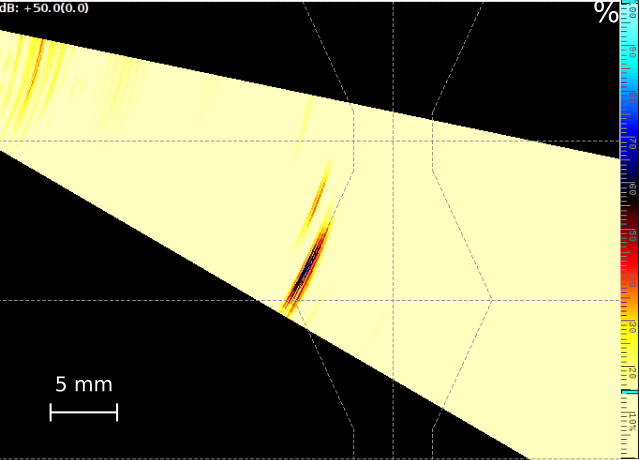
\includegraphics[width=\textwidth]{me_figs/def1.png}
\caption{Fissure --- Copie d'écran}
\end{subfigure}~%
\begin{subfigure}{0.55\textwidth}
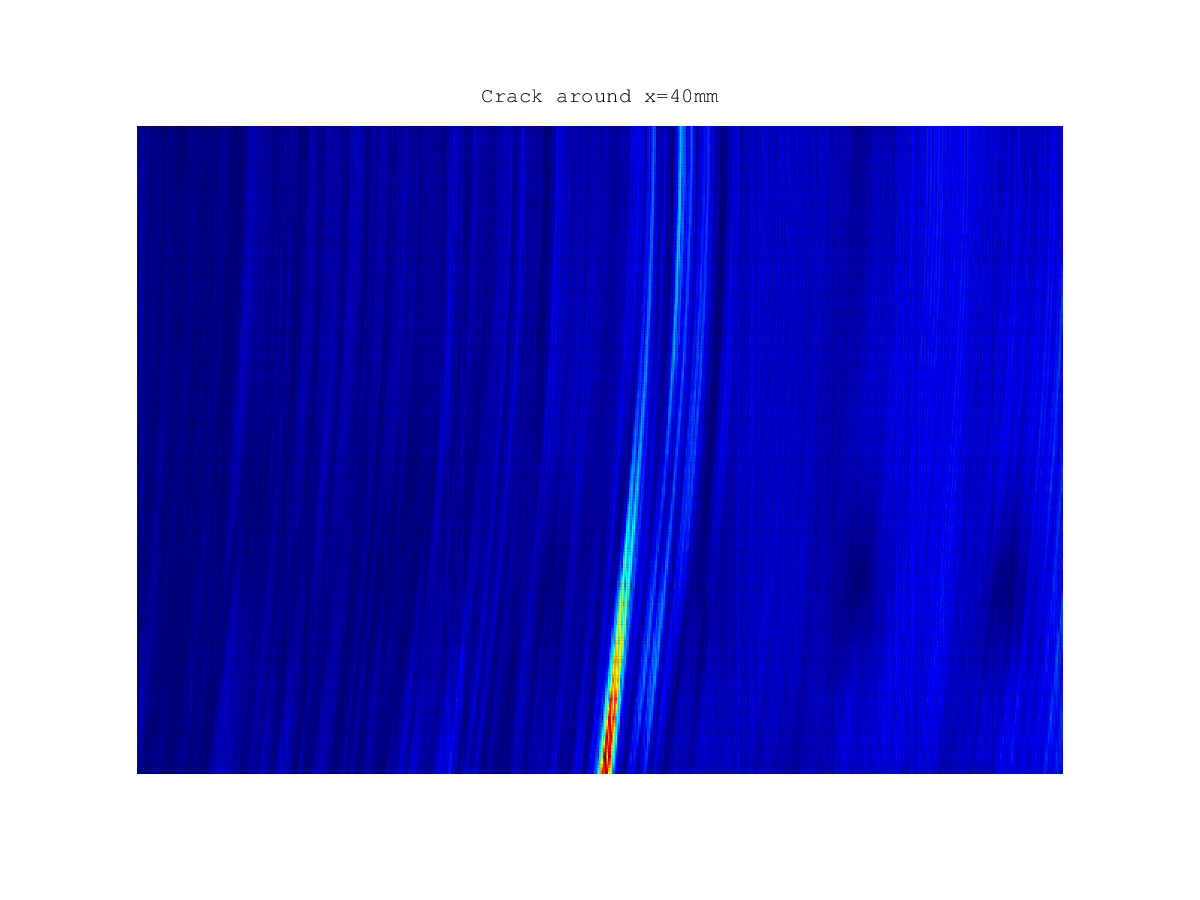
\includegraphics[width=\textwidth]{me_figs/crack_measure.png}
\caption{Fissure --- Données brutes}
\end{subfigure}\\
\begin{subfigure}{0.43\textwidth}
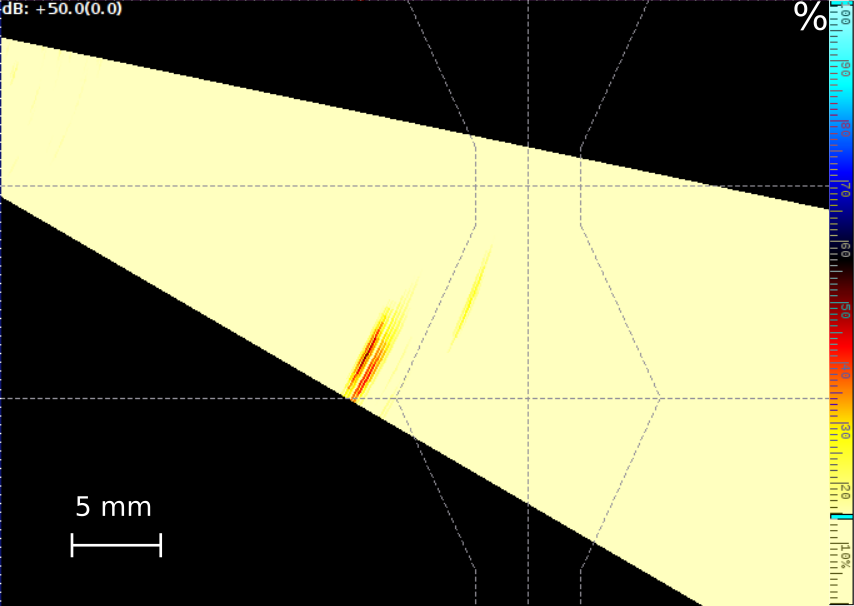
\includegraphics[width=\textwidth]{me_figs/def2.png}
\caption{Porosité --- Copie d'écran}
\end{subfigure}~%
\begin{subfigure}{0.55\textwidth}
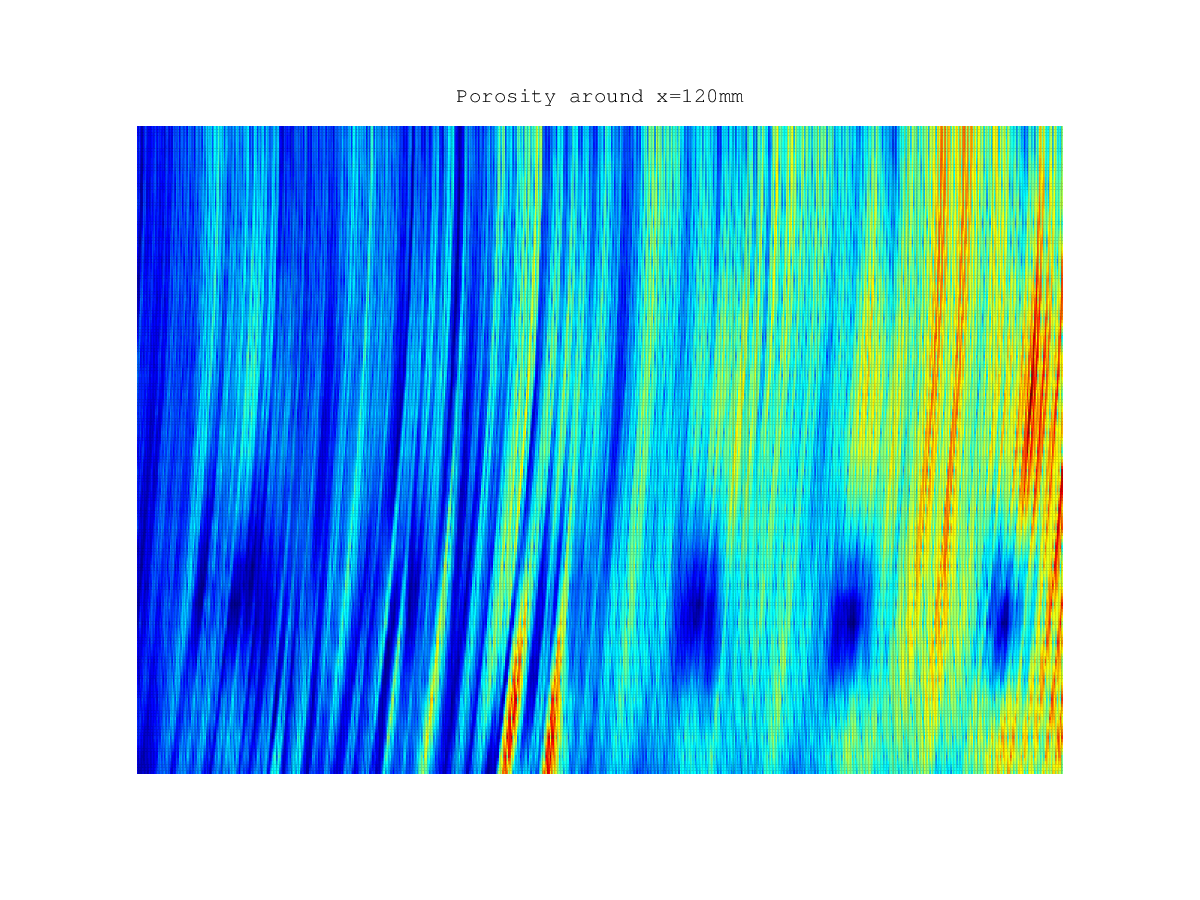
\includegraphics[width=\textwidth]{me_figs/porosity_measure.png}
\caption{Porosité --- Données brutes}
\end{subfigure}\\
\begin{subfigure}{0.43\textwidth}
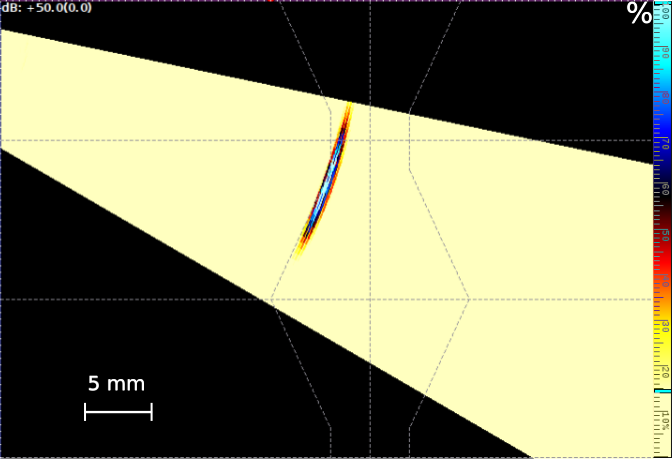
\includegraphics[width=\textwidth]{me_figs/def3.png}
\caption{Manque de fusion --- Copie d'écran}
\end{subfigure}~%
\begin{subfigure}{0.55\textwidth}
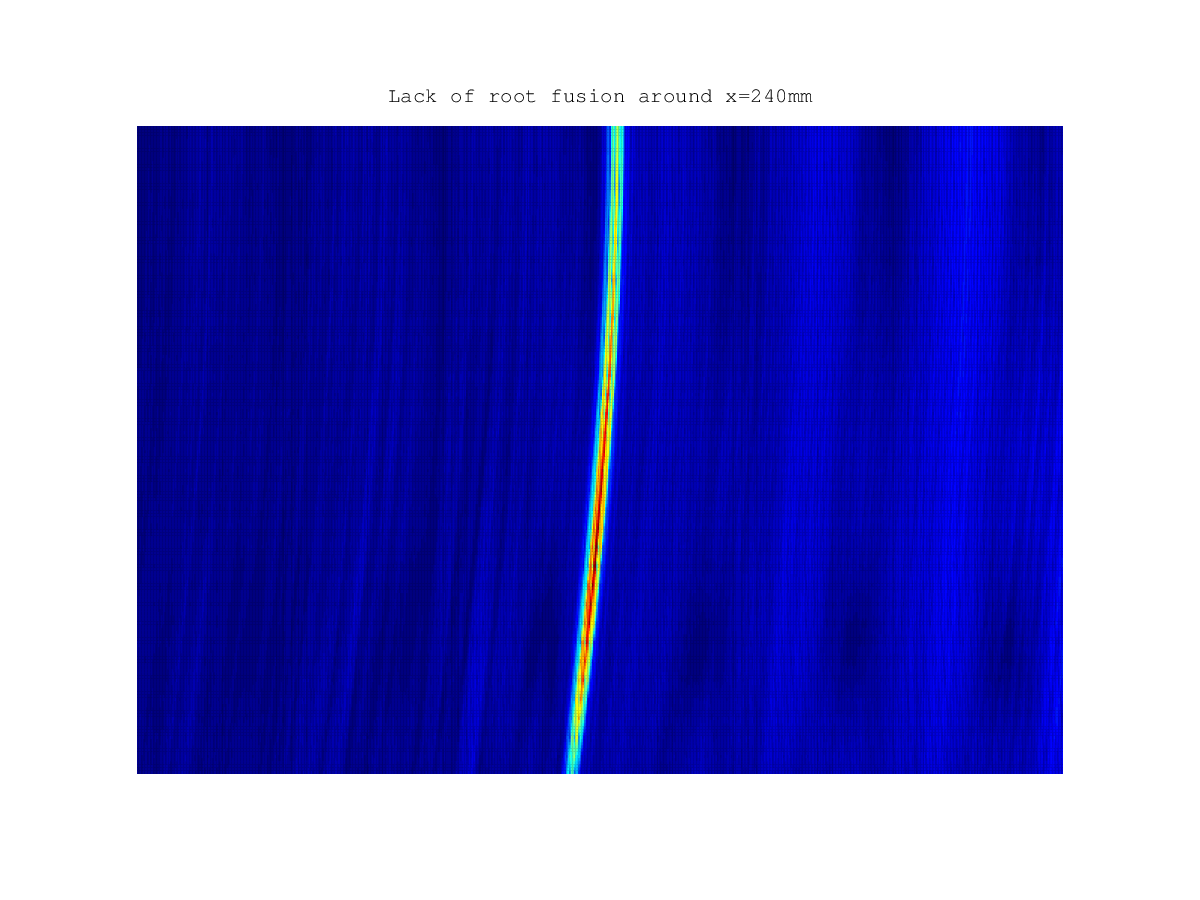
\includegraphics[width=\textwidth]{me_figs/fusion_measure.png}
\caption{Manque de fusion --- Données brutes}
\end{subfigure}\\
\caption{Images obtenues lors de l'inspection. A gauche des copies d'écran du boîtier de contrôle au niveau des défauts (réalisées par A. Dinsenmeyer et T. Lechat) ; à droite, l'affichage des mêmes défaut à partir des données extraites dans GNU/Octave.\label{me:measures}}
\end{figure*}

\subsection{Localisation}

Lors des mesures, les défauts ont été localisés dès le premier scan et les emplacements correspondaient parfaitement à ceux indiqués par la documentation de la pièce d'essai.

Des scans plus localisés ont permis de caractériser aussi bien le type de défaut que son étendue et ce pour chacun des 3 cas.

Les techniques multi-éléments, si elles demandent un réglage et une analyse plus complète, permettent de vraiment représenter les défauts et de les caractériser avec une grande précision.

\section*{Conclusion}

Cette séance a permis de comprendre le fonctionnement des transducteurs multi-éléments et leur intérêt dans le contrôle non-destructif.

Les possibilités de choix du motif de focalisation et de son éventuel déplacement font des méthodes multi-éléments un outil très puissant.

Ces avantages immenses sont malheureusement contre-balancés par le prix élevé des capteurs et des boîtiers d'acquisition et la difficulté de prise en main.

Comme beaucoup de techniques dans le domaine du contrôle, l'expérience et le savoir-faire de l'opérateur joue un rôle non négligeable.


\newpage
\printbibliography

%\appendix
%\input{annexes.tex}
\end{document}
